
%%%%%%%%%%%%%%%%%%%%%%%%%%%%%%%%%%%%%%%%%%%%%%%%%%%%%%%%%%%%%%%%%%%%%%%
%                           Second Chapter                            %
%                  Extensions of Posture Generation                   %
%%%%%%%%%%%%%%%%%%%%%%%%%%%%%%%%%%%%%%%%%%%%%%%%%%%%%%%%%%%%%%%%%%%%%%%

\chapter{Extensions of Posture Generation}
\label{cha:extensions_of_posture_generation}

\graphicspath{{Chapter3-Extensions/Figs/}{Chapter3-Extensions/Figs/IROS14/}}

%Intro
In this chapter, we present three different and unrelated contributions to the state of the art of posture generation.
First, we present a novel method called Integration of Non-Inclusive Contacts in Posture Generation that was published in~\cite{brossette:iros:2014}.
Second, we present a generic algorithm to compute efficiently the derivative of the joint torques of a robot.
Third, we present our endeavor to apply an optimization method called `Lifted Newton Method', presented in~\cite{Albersmeyer:2010:LNM:1958447.1958472}, to problems of inverse kinematics.

%{{{ SECTION: List of contributions

%\section{List of contributions}
%%%%%%%%%%%%%%%%%%%%%%%%%%%%%%%%%%%%%%%%%%%%%%%%%%%%%%%%%%%%%%%%%%%%%%%%

%%                  SECTION LIST OF CONTRIBUTIONS                      %
%%%%%%%%%%%%%%%%%%%%%%%%%%%%%%%%%%%%%%%%%%%%%%%%%%%%%%%%%%%%%%%%%%%%%%%%

%\begin{itemize}
  %\item The method presented before is limiting in many cases. Ladder, stairs climbing\dots.
%Sometimes it is not possible to ensure inclusion of 2 surfaces.
  %\item Contact geometry formulation
    %\begin{itemize}
      %\item Discretisation of contact surfaces for practical reasons
      %\item Contact generation with convex surface inclusions
%Usual methods for generating surface contact are based on point-to-point sampling, on rectangular inclusion, or other limiting methods. We extend that to the inclusion of convex surfaces.
      %\item Inclusive contacts are no problem
      %\item Non-Inclusive contacts lead to non-constant number of constraints or non-smooth gradients, cannot be solved with usual solvers with that formulation
    %\end{itemize}
  %\item{Non inclusive contact constraints}
    %\begin{itemize}
      %\item {Main Idea: Inserting an ellipse in the intersection of polygons}
      %\item {Pseudo-distance (to simplify the formulation)}
      %\item {Modification of the optimization problem}
      %\item {Maximization of the contact area}
      %\item {Using non inclusive contact to maintain stability}
      %\item {Extension to singular cases}
    %\end{itemize}
  %\item{Simulation Results}
    %\begin{itemize}
      %\item{Inclined ladder climbing}
      %\item{Vertical ladder climbing}
      %\item{Climbing Stairs}
      %\item{Walking along a path made of small objects}
    %\end{itemize}
  %\item{Application to ladder climbing (cf. Joris papers)}
%\end{itemize}

%\paragraph{Torque Derivation}

%\paragraph{On the use of lifted variables for Robotics Posture Generation}
%\begin{itemize}
  %\item {Introduction: `J. Albersmeyer and M. Diehl, The lifted Newton Method and its Application in Optimisation'}
  %\item {Lifting Algorithm: Introduce additional variables to reduce the complexity/degree of the equations to solve. And then use a trick to re-condense the system and avoid loosing computation time}
  %\item {Optimization on lifted variables}
  %\item {Condensed BFGS update}
  %\item {Results, experimentation}
  %\begin{itemize}
    %\item Symbolic Inverse Kinematics
    %\item Automatic Lifting algorithm adapted to posture generation
    %\item Several Solvers for lifted and non-lifted systems (Gauss-Newton, SQP, lifted Newton\ldots)
    %\item Compared many optimization methods (Globalization, regularization\ldots)
    %\item Never managed to get results faster than basic methods
  %\end{itemize}
  %\item{Motivation:Development of a posture generator with a specialized solver}
    %\begin{itemize}
      %\item Problem
        %\begin{itemize}
          %\item Robotics problems solved with generic solvers (IPOPT, CFSQP, fmincon\ldots)
          %\item Robotics problems (especially posture generation) are very specific (Constraints, costs, working spaces, sizes\ldots)
        %\end{itemize}
      %\item Solution
        %\begin{itemize}
          %\item Develop a posture generator, along with a nonlinear solver
          %\item Better understanding of our own solver
          %\item Ability to use the solver in new ways:
          %\begin{itemize}
            %\item Working on Manifolds
            %\item Variable numbers of constraints
            %\item Automatic management of variables, constraints and mathematical expressions
          %\end{itemize}
        %\end{itemize}
    %\end{itemize}
%\end{itemize}
%}}}
\section{Integration of Non-Inclusive Contacts in Posture Generation}
\label{sec:integration_on_non_inclusive_contacts_in_posture generation}

%%%%%%%%%%%%%%%%%%%%%%%%%%%%%%%%%%%%%%%%%%%%%%%%%%%%%%%%%%%%%%%%%%%%%%%%%
%  SECTION INTEGRATION ON NON-INCLUSIVE CONTACTS IN POSTURE GENERATION  %
%%%%%%%%%%%%%%%%%%%%%%%%%%%%%%%%%%%%%%%%%%%%%%%%%%%%%%%%%%%%%%%%%%%%%%%%%

In Section~\ref{sec:contact_constraints}, we defined a set of constraints (equations~\Eqref{eq:coplanarity}) that ensures the coplanarity of two planar surfaces in a geometric contact.
Those equations guarantee the coplanarity of two infinite planar surfaces.
Another set of constraints needs to be added to ensure the validity of a contact between two bounded surfaces $S_1$ and $S_2$, to ensure that their intersection is not empty and that it is large enough to support the contact.

We propose a simple way to formulate geometric contact formation to have an arbitrary intersection shape that we apply to a robotic (humanoid) posture generation problem, when searching for a contact between two surfaces.
We start by defining convex areas of contact on the robot's body and the environment, that we call \emph{contact patches}.
We can generate contacts with an arbitrary intersection of a pair of any of these predefined contact patches.
Virtually any planar surface can be a contact patch.
In our group's previous works, the constraints formulating a new contact in the posture generator, states that a contact patch is totally included into another, which is obviously a limitation of the posture generation.
A simple example is when a human climbs stairs.
S/he usually contacts only the front half of its foot with each step, the heel almost never touches the steps.
Our new geometric contact modeling writes very simply as additional constraints and variables added to the optimization problem.
It consists of searching for an ellipse inscribed in the intersection of the pair of patches we want in contact.
The result of our posture generator is then a configuration where contact patches are not necessarily included in one another (therefore we named it non-inclusive) and the shape and area of their intersection can be monitored.
This allows our posture generator to propose contacts of different shapes with a non-predefined number of contact points (used later to compute reaction/contact forces).
We illustrate the efficiency of our method in multi-contact posture generation with the HRP-2 and ATLAS humanoid robots with results that can not be generated automatically by existing methods.

\begin{figure}
\centering
  \centering
  \setlength\fboxsep{0pt}
  \setlength\fboxrule{1pt}
  \fbox{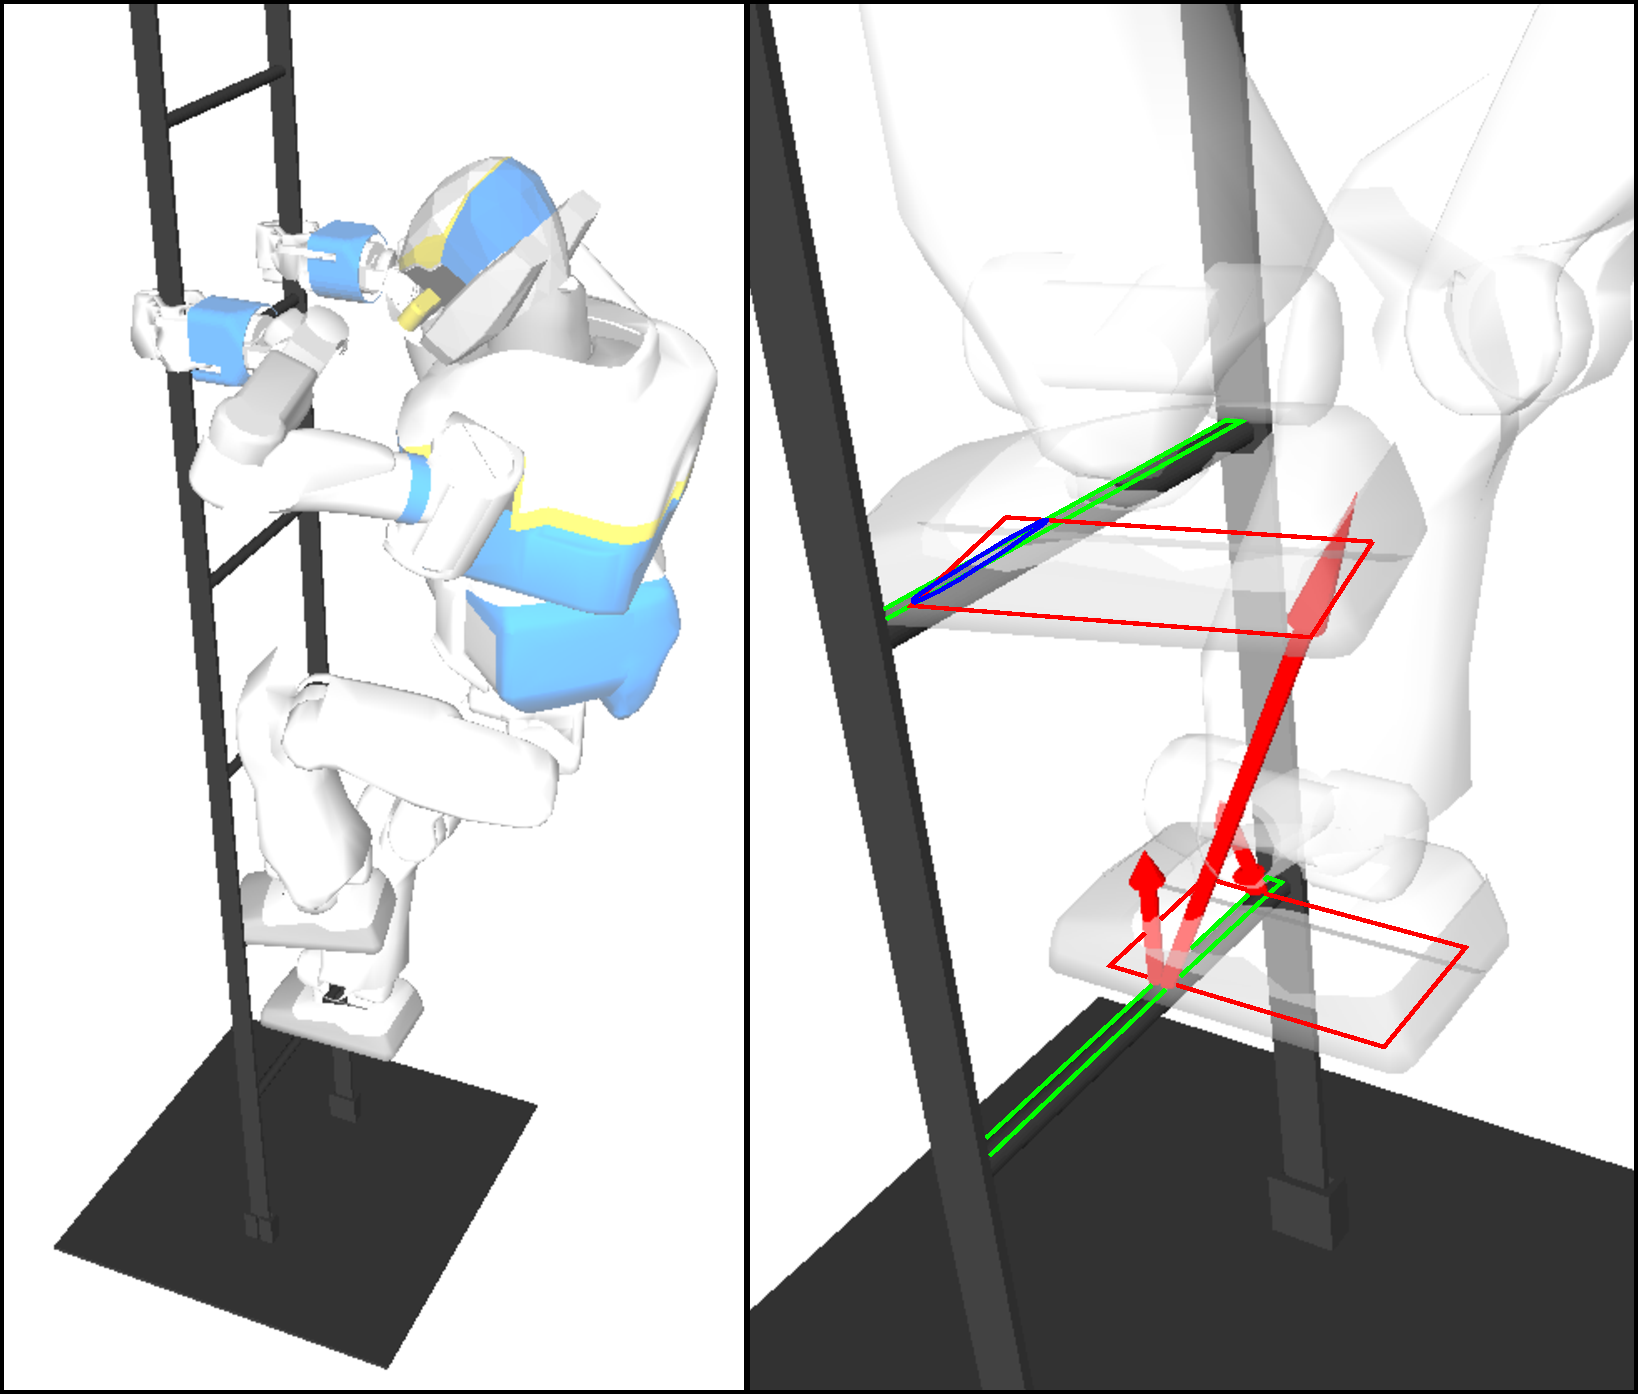
\includegraphics[width=.55\linewidth]{hrp2_ladder_jrl_5_combo.pdf}}
\caption{Using non-inclusive contacts for ladder climbing (green/red: contact polygons; blue: contact ellipse; red arrows: contact forces resultants)}
\label{fig:hrp2_jrl_complete}
\end{figure}

%In general, desired contacts write as hard constraints to fulfill in an optimization problem.
%Yet, we need to write the maths for, say, put the gripper on the wall and the left foot on the ground.
%In general, the maths of a gripper is a complex geometric description, so is often that of the environment.
A contact is generally defined by a pair of points (one on each object in contact) and a normal vector.
A contact constraint consists in finding a posture in which the predefined authorized contact points and normal of each body match~\cite{zhang:TePRA:2013}\cite{hauser:ijrr:2008}.
Likewise, in~\cite{osswald:iros:2011}, the position of the feet of the NAO robot is manually tuned in order to obtain statically stable position during the climbing of a spiral staircase.
In~\cite{Chestnutt:2009:BNR:1733023.1733314}, the surface in contact is chosen according to two criteria: the position of the force sensors of the feet, and the desired type of contact.
In~\cite{sentis:itro:2010}, the problem of contact discovery in not considered.
In~\cite{mordatch:acm:2012}, two surfaces are considered in contact as soon as the center point of one of them touches the other one and their normals match.
Although used in many papers, it is not difficult to see that this definition of contact excludes a series of possibilities that would have been obtained if the predefined points were placed in different configurations within their respective patches.
Table~\ref{tbl:contact_description} presents some diagrams describing some typical methods used for constraining the relative positions of contact surfaces.
On each figure, the blue rectangle describes a surface $S_2$ with which we want to make contact with surface $S_1$.
$S_1$ is drawn in green if the contact is valid and in red otherwise.

\begin{table}[ht!]
  \centering
  \begin{tabular}{c m{8cm}}
    \toprule
    \begin{minipage}{.4\textwidth}
      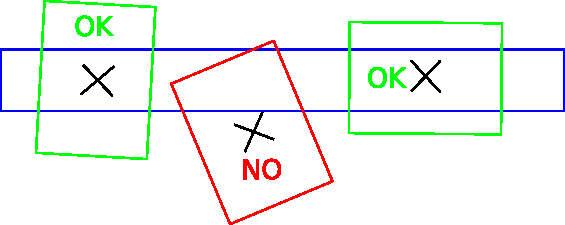
\includegraphics[width=0.9\linewidth]{contact1.pdf}
    \end{minipage}
    &
    %\begin{minipage}[t]{5cm}
    The center point of $S_1$ is included
    in $S_2$~\cite{hauser:humanoid:2005}
    \begin{itemize}
      \item Easy and cheap to compute
      \item Eliminates valid solutions
    \end{itemize}
    %\end{minipage}
    \\ \midrule
    \begin{minipage}{.4\textwidth}
      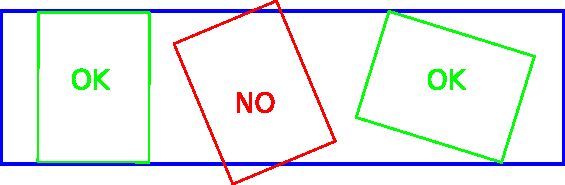
\includegraphics[width=0.8\linewidth]{contact2.pdf}
    \end{minipage}
    &
    %\begin{minipage}[t]{5cm}
    $S_1$ is fully included in $S_2$~\cite{bouyarmane:ar:2012}
    \begin{itemize}
      \item Eliminates many valid solutions
    \end{itemize}
    %\end{minipage}
    \\ \midrule
    \begin{minipage}{.4\textwidth}
      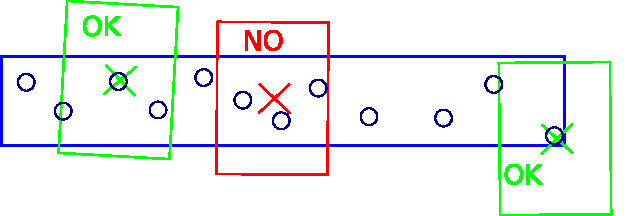
\includegraphics[width=\linewidth]{contact3.pdf}
    \end{minipage}
    &
    %\begin{minipage}[t]{5cm}
    $S_1$ contains a set of sampled points, the center of $S_2$ has to match one of them~\cite{chestnutt:humanoids:2003}
    \begin{itemize}
      \item Discrete set of possible solutions
      \item Eliminates many valid solutions
    \end{itemize}
    %\end{minipage}
    \\ \midrule
    \begin{minipage}{.4\textwidth}
      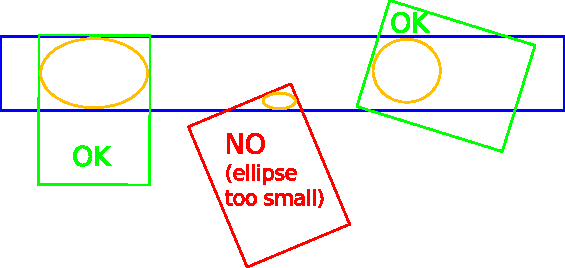
\includegraphics[width=0.9\linewidth]{contact4.pdf}
    \end{minipage}
    &
    %\begin{minipage}[t]{5cm}
    The contact is valid if an ellipse of sufficient size is found in
    the intersection $S_1 \cap S_2$~\cite{brossette:iros:2014}
    \begin{itemize}
      \item Smooth
      \item Does not eliminate valid solutions
    \end{itemize}
    %\end{minipage}
    \\ \bottomrule
  \end{tabular}
  \caption{Contact descriptions}
\label{tbl:contact_description}
\end{table}

In planning, once a geometric contact is found for a posture, the next posture will make use of it as a stability contact and apply forces on it.
Once the geometric contact is established, one determines the intersection of the contacting surfaces in order to find the points on which the reaction forces are to be computed when the geometric contact becomes a stability contact.
Several approaches require fixing the number of contact points or to have inclusive contact (i.e.\ one patch is fully included in the other)~\cite{bouyarmane:ar:2012}.

We provide a simple solution that relaxes contact constraints and gets rid of predefining the contact points.
We consider that a contact is valid if the intersection between two distinct patches has an area greater than a given threshold.
To enforce this, we require this intersection to contain an ellipse whose surface can possibly be maximized.
Convex patches allow writing the inscription constraints easily by means of half-spaces.


\subsection{Contact geometry formulation}
\label{subsec:contact_geometry_formulation}

%%%%%%%%%%%%%%%%%%%%%%%%%%%%%%%%%%%%%%%%%%%%%%%%%%%%%%%%%%%%%%%%%%%%%%%
%              SUBSECTION CONTACT GEOMETRY FORMULATION                %
%%%%%%%%%%%%%%%%%%%%%%%%%%%%%%%%%%%%%%%%%%%%%%%%%%%%%%%%%%%%%%%%%%%%%%%

%For our formulation, we consider a situation where a set of contacts between the robot and its environment are already made, and therefore fixed, and we want to add a new contact to this set.
%This doesn't induce any loss of generality since it just comes down to adding the contacts one by one.
%To ensure that the new contact can be reached in a quasi-static way, we look for a configuration where the new contact is a geometric contact.
%Let us consider that the contact to add is defined by two flat surfaces $S_1$ and $S_2$ which are respectively delimited by two convex polygons $P_1$ and $P_2$.
Let us consider a contact defined by two flat surfaces $S_1$ and $S_2$ which are respectively two convex polygons $P_1$ and $P_2$.
For this contact to be valid, it is necessary that the intersection $P_1 \cap P_2$ is not empty.
%We propose a method in which the size of the contact area is approximated by the size of an ellipse that is inscribed in it.
%If such an ellipse is found and is of a sufficient size, then the contact is valid.
%This allows considering contacts between surfaces that do not necessarily include each other.

An important remark is that the number of sides of the intersection polygon is not known a priori and, as shown in~\Figref{fig:polygon-inter}{}, this number can change depending on the configuration.
Each time this number changes, the gradient of the area of the intersection is discontinuous.
This is an issue for integrating any constraint or objective based on the area because we use a solver for smooth optimization problems.
This issue could be dealt with by using non-smooth optimization algorithms, but such algorithms are slower and less available, and our posture generator is not designed to use them.
\begin{figure}[!htb]
  \centering
  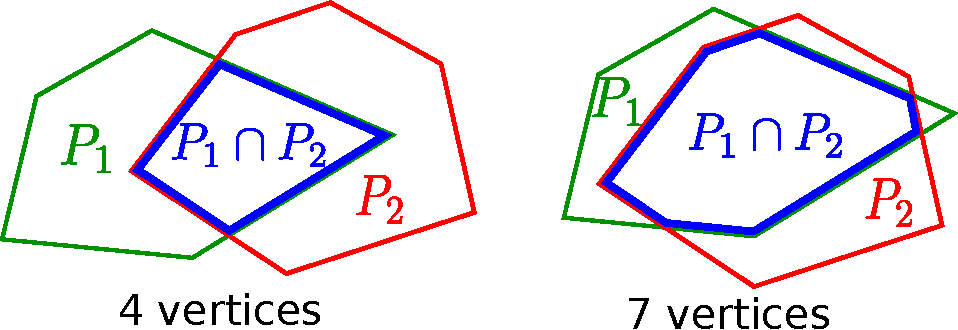
\includegraphics[width=0.6\columnwidth]{polygon-inter.pdf}
  \caption{Topological instability of $P_1 \cap P_2$}
\label{fig:polygon-inter}
\end{figure}
Moreover, supposing that we want to write constraints based on the sides of the contact area, then, the number of constraints would change with the number of vertex of $P_1 \cap P_2$.
The large majority of the optimization software cannot deal with a non-constant number of constraints.
The solution proposed in Section~\ref{subsec:ellipse} overcomes these issues by defining a set of constraints that is independent of the topology of the intersection area.



\subsection{Non-inclusive contact constraints}
\label{subsec:ellipse}

%%%%%%%%%%%%%%%%%%%%%%%%%%%%%%%%%%%%%%%%%%%%%%%%%%%%%%%%%%%%%%%%%%%%%%%
%          SUBSECTION NON-INCLUSIVE CONTACT CONSTRAINTS               %
%%%%%%%%%%%%%%%%%%%%%%%%%%%%%%%%%%%%%%%%%%%%%%%%%%%%%%%%%%%%%%%%%%%%%%%



\subsubsection{Main Idea}
\label{subsubsec:idea}

%%%%%%%%%%%%%%%%%%%%%%%%%%%%%%%%%%%%%%%%%%%%%%%%%%%%%%%%%%%%%%%%%%%%%%%
%                      SUBSUBSECTION MAIN IDEA                        %
%%%%%%%%%%%%%%%%%%%%%%%%%%%%%%%%%%%%%%%%%%%%%%%%%%%%%%%%%%%%%%%%%%%%%%%

We propose a smooth formulation of the non-empty intersection between two contact surfaces.
We assume that co-planarity of $S_1$ and $S_2$ is obtained by using the constraints presented in~\Eqref{eq:coplanarity}.
Here we focus on the intersection of the two polygons $P_1$ and $P_2$, respectively describing the contours of $S_1$ and $S_2$.
%As we pointed out earlier, a problem with computing the area of intersection of two polygons comes from the fact that depending on their positions in space, the number of edges of their intersection can change (cf.~\Figref{fig:polygon-inter}{}), which induces discontinuity of the gradient of the area and change of the number of constraints associated with this contact.

To avoid dealing with changes of topology, we consider using an ellipse $\mathcal{E}$ included in $P_1 \cap P_2$ to estimate the area of the intersection.
Since $P_1$ and $P_2$ are convex polygons, then $P_1 \cap P_2$ is also a convex polygon.
A convex polygon can be seen as an intersection of half-planes based on the lines supporting its edges.
Thus, an ellipse is inside of a convex polygon if it lies entirely in the corresponding half-planes.
Having the ellipse be included in the intersection of two polygons is equivalent to having it included in both polygons:
\begin{equation}
\mathcal{E} \subset P_1 \cap P_2 \ \Longleftrightarrow \
\mathcal{E} \subset P_1 \ \ \text{AND} \ \  \mathcal{E} \subset P_2
\end{equation}
Even if the number of edges of $P_1 \cap P_2$ can change, the numbers of edges of $P_1$ and $P_2$ respectively are fixed.
%\begin{wrapfigure}{r}{0.4\columnwidth}
%  \begin{center}
%    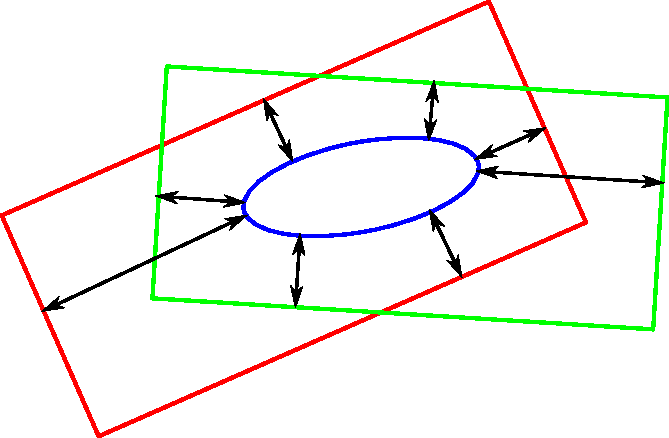
\includegraphics[width=0.4\columnwidth]{distance.pdf}
%    \caption{Distance ellipse-polygons}
%  \end{center}
%  \label{fig:distance}
%\end{wrapfigure}
%Therefore, if we ensure that the ellipse $\mathcal{E}$ is on the left side of each segment defining $P_1$ and $P_2$, then it is inside $P_1 \cap P_2$.
To assert that an ellipse lies in a half-plane, we need a function that is positive when the ellipse is in it (with zero value when the ellipse is on the edge) and negative otherwise.
The signed distance to the line defining the half-space is a good candidate (distance ellipse-line if the ellipse is in the half-plane, opposite of the penetration distance if not), but actually, any pseudo-distance does the job.
And a sufficient condition for the ellipse to be inside the polygons intersection is that the pseudo-distance between the ellipse and each edge of both polygons is positive (see~\Figref{fig:distance}{}).
By considering each edge separately as opposed to the pseudo-distance of the ellipse to a whole polygon, we can write smooth constraints with a simple pseudo-distance function.
We develop such a pseudo-distance in what follows.
%In order to measure the fact that a point is on the left side of an oriented segment we use a signed distance $d_s$, this signed distance is positive and equal to a usual distance when the point is on the left side of the segment and is negative and equal to the opposite of the usual distance when the point is on the right side of the segment.
% and algorithm~\ref{alg:ellipse-in-intersection} where $d_s$ stand for the pseudo-distance.
%\begin {algorithm}
%\caption{Inclusion of ellipse $\mathcal{E}$ in polygon intersection}
%\begin{algorithmic}
%\STATE {Let $P_1$ and $P_2$ be two coplanar convex polygons}
%\STATE {Let {\bf V} be an empty vector}
%\FORALL{Edge E in $P_1$}
%\STATE {Add $d_s(\mathcal{E}, E)$ to {\bf V}}
%\ENDFOR
%\FORALL{Edge E in $P_2$}
%\STATE {Add $d_s(\mathcal{E}, E)$ to {\bf V}}
%\ENDFOR
%\IF {{\bf V}$\succ 0$ (all terms of {\bf V} are positive)}
%\STATE {Return $\mathcal{E} \subset P_1 \cap P_2$}
%\ELSE
%\STATE {Return $\mathcal{E} \not\subset P_1 \cap P_2$}
%\ENDIF
%\end{algorithmic}
%\label{alg:ellipse-in-intersection}
%\end{algorithm}
%
\begin{figure}[!htb]
  \centering
  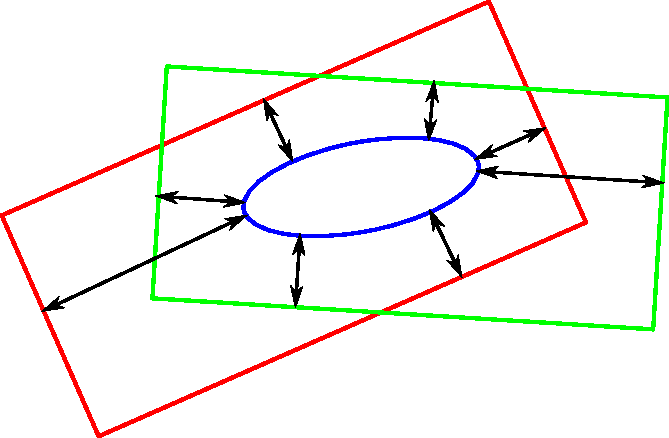
\includegraphics[width=0.4\columnwidth]{distance.pdf}
  \caption{Distance between $\mathcal{E}$ and $P_1 \cap P_2$.}
\label{fig:distance}
\end{figure}

\subsubsection{Pseudo-distance}
\label{subsubsec:formulation}

%%%%%%%%%%%%%%%%%%%%%%%%%%%%%%%%%%%%%%%%%%%%%%%%%%%%%%%%%%%%%%%%%%%%%%%
%                   SUBSUBSECTION PSEUDO-DISTANCE                     %
%%%%%%%%%%%%%%%%%%%%%%%%%%%%%%%%%%%%%%%%%%%%%%%%%%%%%%%%%%%%%%%%%%%%%%%

%To estimate the constraint of inclusion of the ellipse $\mathcal{E}$ in both polygons $P_1$ and $P_2$, we need to compute the signed distance between $\mathcal{E}$ and each segment of the polygons.
Computing the distance between an ellipse and a line is not straightforward, whereas the distance between a line and a circle is very easy to compute.
Also, we note that in the frame $F_\mathcal{E}$ defined by the ellipse's axes and pseudo-radius, the ellipse is a circle of radius $r_{\mathcal{E}}=1$ (The x-unit along the first axis of the ellipse is $r_x$, the first radius of the ellipse, the y-unit along the second axis of the ellipse is $r_y$, the second radius).
The transformation from the original frame $F_0$ in which the ellipse and the polygons are described to the ellipse's frame $F_\mathcal{E}$ is just the composition of a rotation and a scaling of the space along the axes of the ellipse with a scaling vector $[\frac{1}{r_x}, \frac{1}{r_y}]$.
The effect of such a transformation applied to an ellipse and two polygons is shown in~\Figref{fig:pseudo-distance}{}.
%Also, those transformations will not modify the validity of our constraint, indeed, the distance between $\mathcal{E}$ and any segment $E$, computed in $F_\mathcal{E}$, is a pseudo-distance in $F_0$.
%Therefore, we still get all the information needed to ensure the inclusion of $\mathcal{E}$ in $P_1 \cap P_2$.
We thus defined the following pseudo-distance from an ellipse to a half-plane as the signed Euclidean distance from the corresponding unit circle to the transformed half-plane in the frame $F_\mathcal{E}$.

\begin{figure}[!htb]
  \centering
  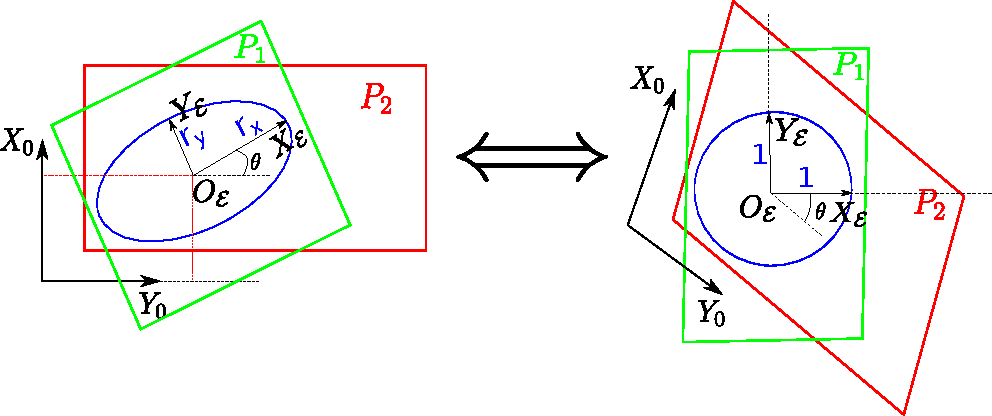
\includegraphics[width=0.9\linewidth]{pseudo-distance.pdf}
  \caption{Transformation from $F_0(O_0, X_0, Y_0)$ to $F_\mathcal{E}(O_\mathcal{E},X_\mathcal{E},Y_\mathcal{E})$}
\label{fig:pseudo-distance}
\end{figure}

Now let us consider a single segment $p_i p_j$ and an ellipse $\mathcal{E}$ defined in $F_0$.
The expression of a vector ${{\bf v}_{F_0}}^T = {[v_x, v_y]}_{F_0}$ in $F_\mathcal{E}$ is obtained by applying the formula~\Eqref{eq:F0-to-FE}.
\begin{equation}
{\bf v}_{F_\mathcal{E}} =
\begin{bmatrix}
\frac{1}{r_x} & 0 \\
0 & \frac{1}{r_y}
\end{bmatrix}
\cdot \begin{bmatrix}
\cos(\theta) & \sin(\theta) \\
-\sin(\theta) & \cos(\theta)
\end{bmatrix}
\cdot {\bf v}_{F_0}
\label{eq:F0-to-FE}
\end{equation}
In $F_\mathcal{E}$, the distance between the circumference of $\mathcal{E}$ and the segment $p_i p_j$ is:
\begin{equation}
  d_s(\mathcal{E}, p_i p_j) = \frac{{\left.\overrightarrow{p_i p_j}\right|}_{F_\mathcal{E}} \wedge {\left.\overrightarrow{p_i O_\mathcal{E}}\right|}_{F_\mathcal{E} } }{\| \overrightarrow{p_i p_j}\|_{F_\mathcal{E} } }-1
\end{equation}
where $\wedge$ denotes the cross product and $O_{\mathcal{E}}$ is the center of the ellipse.

To avoid numerical problems when the segment $p_i p_j$ is small, it is preferable to multiply this distance by $\| \overrightarrow{p_i p_j}\|_{F_\mathcal{E}}$ before using it as a constraint.
Then we get the following constraint:
\begin{equation}
  -{\left.\overrightarrow{p_i p_j}\right|}_{F_\mathcal{E}} \wedge {\left.\overrightarrow{p_i O_\mathcal{E}}\right|}_{F_\mathcal{E}}+\| \overrightarrow{p_i p_j}\|_{F_\mathcal{E}} \leq 0
\label{eq:pseudo-distance}
\end{equation}

The combination of these equations~\Eqref{eq:F0-to-FE} and \Eqref{eq:pseudo-distance} applied for each edge of the polygons gives us all the necessary tools to develop a set of constraints that ensures that an ellipse is inside the intersection of two polygons.



\subsubsection{Modification of the optimization problem}

%%%%%%%%%%%%%%%%%%%%%%%%%%%%%%%%%%%%%%%%%%%%%%%%%%%%%%%%%%%%%%%%%%%%%%%
%       SUBSUBSECTION MODIFICATION OF THE OPTIMIZATION PROBLEM        %
%%%%%%%%%%%%%%%%%%%%%%%%%%%%%%%%%%%%%%%%%%%%%%%%%%%%%%%%%%%%%%%%%%%%%%%

To include the above idea in our posture generation, we need to modify the optimization problem~\Eqref{eq:PG} as follows.
Each non-inclusive geometrical contact adds five variables to the optimization vector, corresponding to the position, orientation, and radiuses of the ellipse ($x$, $y$, $\theta$, $r_x$ and $r_y$).
One constraint of ellipse inclusion (as described above) is added to the problem for each edge of the polygons.
The parameters $r_x$ and $r_y$ are given lower positive bounds to ensure that the ellipse is not empty.
The existence of a contact between $S_1$ and $S_2$ is thus transformed into the existence of $r_x$ and $r_y$ respecting their bounds.
In summary, this kind of constraint adds 5 variables and $card(P_1)+card(P_2)$ constraints to the optimization problem (where $card(P)$ denotes the number of edges of polygon $P$), while the `usual' inclusion constraint adds 0 variable and $card(P_1)card(P_2)$ constraints.
The existence of the contact can alternatively be enforced by imposing a minimum area for the ellipse.



\subsubsection{Maximization of the contact area}
\label{subsubsec:optim-ellipse-area}

%%%%%%%%%%%%%%%%%%%%%%%%%%%%%%%%%%%%%%%%%%%%%%%%%%%%%%%%%%%%%%%%%%%%%%%
%           SUBSUBSECTION MAXIMIZATION OF THE CONTACT AREA            %
%%%%%%%%%%%%%%%%%%%%%%%%%%%%%%%%%%%%%%%%%%%%%%%%%%%%%%%%%%%%%%%%%%%%%%%

The formulation in the above section only ensures the existence of a contact of minimal size.
However, one may want to find a contact area as large as possible, so that it is more likely to be able to support strong forces and have strong friction forces, which is helpful to guarantee the stability of the robot.
Therefore, it seems appropriate to try and maximize the area of contact between two polygons.
As explained before, computing the area of the intersection surface is not a good practice in our case.
But the ellipse computed as above gives a lower bound of the contact area.

\begin{equation}
\mathcal{E} \subset P_1 \cap P_2 \Longrightarrow  \mathcal{A}(\mathcal{E}) \le \mathcal{A}(P_1 \cap P_2)
\end{equation}
with $\mathcal{A}(X)$ being the area of $X$.\newline
Therefore, we can maximize the area of the ellipse in order to maximize the contact area.
This is readily obtained by minimizing the value of $f_{\text{ellipse}}(r_x, r_y) = -\pi r_x r_y$ in the modified problem~\Eqref{eq:PG}.
In case there are other cost functions, the above cost can be added to them with a desired weight.
This requires, however, to scale properly the cost so as to have a meaningful and easy-to-tune weight: the range of value of the ellipse's area goes from $0$ to $\mathcal{A}(P_1 \cap P_2) \leq \min (\mathcal{A}(P_1), \mathcal{A}(P_2))$.
This latter quantity can be small (a typical area of contact of a humanoid robot is about $0.01m^2$, some environment surfaces can be smaller).
To get a basic cost (before weighting) of magnitude around $1$, we use the following scaling:
\begin{equation}
f_\text{ellipse}(r_x, r_y) = - \frac{\pi r_x r_y}{\min (\mathcal{A}(P_1), \mathcal{A}(P_2))}
\label{eq:cost-ellipse}
\end{equation}
This cost's absolute value will always be less than $1$, but not much less around the optimum, in most cases.


\subsubsection{Using a non-inclusive contact to maintain stability}
\label{subsubsec:stability}

%%%%%%%%%%%%%%%%%%%%%%%%%%%%%%%%%%%%%%%%%%%%%%%%%%%%%%%%%%%%%%%%%%%%%%%
%  SUBSUBSECTION USING A NON-INCLUSIVE CONTACT TO MAINTAIN STABILITY  %
%%%%%%%%%%%%%%%%%%%%%%%%%%%%%%%%%%%%%%%%%%%%%%%%%%%%%%%%%%%%%%%%%%%%%%%

The method we presented so far allows finding a configuration in which a new non-inclusive contact is added, but this contact does not bear any force.
It is found as a geometrical contact, but will eventually have to bear some forces, and thus, become a stability contact.
Usually, for a stability contact, each vertex of the contact area is considered as the application point of a force that has to be in a friction cone.
Since our method allows dealing with surfaces that are intersecting each other, the contact surface is not known beforehand.
Therefore, as soon as a non-inclusive contact is going to be used for the stability, we compute the intersection of the two polygons $P_1$ and $P_2$ that are involved, and that intersection $P_1 \cap P_2$ is the contact surface, and its vertices will bear the forces.
We do not present here the algorithm to compute the intersection of two convex polygons, as it can be found in the literature easily.
%Since this computation is done outside of the posture generation, it does not imply any numerical problems.

\subsubsection{Extension to singular cases}
\label{subsubsec:singular_cases}
Our method can be extended to be used to approximate singular situations, such as finding an optimal contact with a linear or even punctual surface.
This is done by giving a slight width to the point or the line.
This approximation is physically grounded:
%The main problem with that kind of approach is that it is not possible to deal with a perfectly linear surface, that's why we call "line" a very thin rectangle and "point" a very small square.
in terms of real contacts, linear or punctual contacts do not exist.
In fact, since all objects are deformable, even slightly, the contact area between two objects cannot be a perfect line, and must have a non-null area, which justifies that linear and punctual contacts can be modeled as thin contact surfaces.
By defining such a surface, we impose partly the orientation of the contact.
%A problem we encountered with that extension is that if the contact area is thin, then the ellipse  found inside this area will be thin too and thus have a small area.
%This lead to some conditioning problems and at first the solver would stop without optimizing the size of the ellipse.
%That was due to the fact that the area of the ellipse was negligible compared to the other costs involved in the cost function.
%That is why we divided the area of the ellipse by $\min (\mathcal{A}(P_1), \mathcal{A}(P_2))$ to get the equation~\Eqref{eq:cost-ellipse} in the first place.
Here again, one must be careful with numerical issues.
Dealing with small numbers (here we would like to take the width of a fraction of a centimeter) may induce conditioning problems.
Also, having two close parallel constraints of opposite direction (i.e. $g(x)\leq \alpha$ and  $-g(x)\leq \alpha$ with $\alpha$ small) is not a good practice in optimization as it will lead the solver to take small steps.
Therefore, it is best to apply a scaling to the constraints by applying a geometrical scaling to $P_1$ and $P_2$ in the appropriate direction.\newline
Likewise, constraints on the area of the ellipse should be based on the same formulation as in equation~\Eqref{eq:cost-ellipse}.



\subsection{Simulation results}
\label{subsec:simu}

%%%%%%%%%%%%%%%%%%%%%%%%%%%%%%%%%%%%%%%%%%%%%%%%%%%%%%%%%%%%%%%%%%%%%%%
%                   SUBSECTION SIMULATION RESULTS                     %
%%%%%%%%%%%%%%%%%%%%%%%%%%%%%%%%%%%%%%%%%%%%%%%%%%%%%%%%%%%%%%%%%%%%%%%

In order to illustrate our method, we present some examples starring the HRP-2 and ATLAS humanoid robots, that are typical posture generations encountered in multi-contact planning.
%All the computations of the following experiments are performed on a single thread of an Intel(R) Core(TM) i7-3840QM CPU at 2.80GHz, with 16Go of RAM.
For the implementation of our posture generator, we use the RobOptim optimization framework~\cite{moulard:jsme:2013} relying on the IPOPT solver~\cite{wachter:mathprog:2006}.



\subsubsection{Inclined ladder climbing}
\label{subsubsec:inclined_ladder_climbing}

%%%%%%%%%%%%%%%%%%%%%%%%%%%%%%%%%%%%%%%%%%%%%%%%%%%%%%%%%%%%%%%%%%%%%%%
%               SUBSUBSECTION INCLINED LADDER CLIMBING                %
%%%%%%%%%%%%%%%%%%%%%%%%%%%%%%%%%%%%%%%%%%%%%%%%%%%%%%%%%%%%%%%%%%%%%%%

In this first example, we generate a posture that is part of an inclined ladder climbing planning.
We consider that the robot HRP-2 reached a posture in which its right foot is on the first step and its right hand is grasping the right guardrail, both of those contacts are bearing forces.
Those contacts are fixed, and we search a posture that adds to it a geometrical contact between the left foot and the second step.
We require the contact to include an ellipse with both radiuses bigger than 40\% of the ladder step's width.
The resulting posture and a close-up view of the contact areas are shown in~\Figref{fig:hrp2_darpa_complete}{}.
The latter shows clearly how an ellipse of sufficient size is found, included in the contact area between the left foot and the second step.
It also shows that the contact forces on the right foot are located on the vertex of the intersection of the contact surfaces between the right foot and the first step, which was also generated with our method, in a prior posture generation.
One can note that we use a contact area slightly smaller than the actual surface under the foot of the robot.
We use indeed safety margins to account for modeling errors so that the obtained posture is achievable by the real robot.
%\begin{figure*}
%\centering
%\begin{subfigure}{.5\textwidth}
%  \centering
%  \setlength\fboxsep{0pt}
%  \setlength\fboxrule{1pt}
%  %\fbox{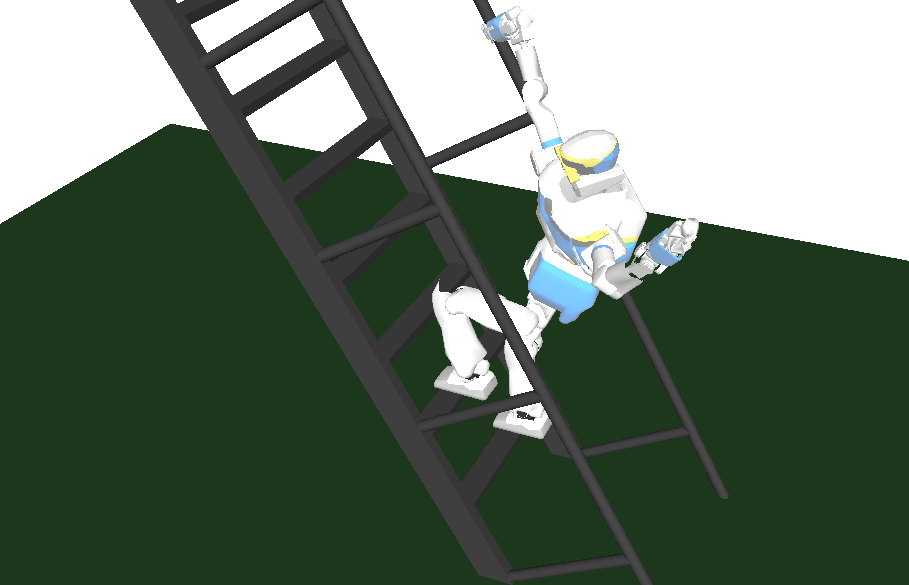
\includegraphics[width=\linewidth]{papers/IROS2014/figure/hrp2_ladder_darpa.png}}
%  %\fbox{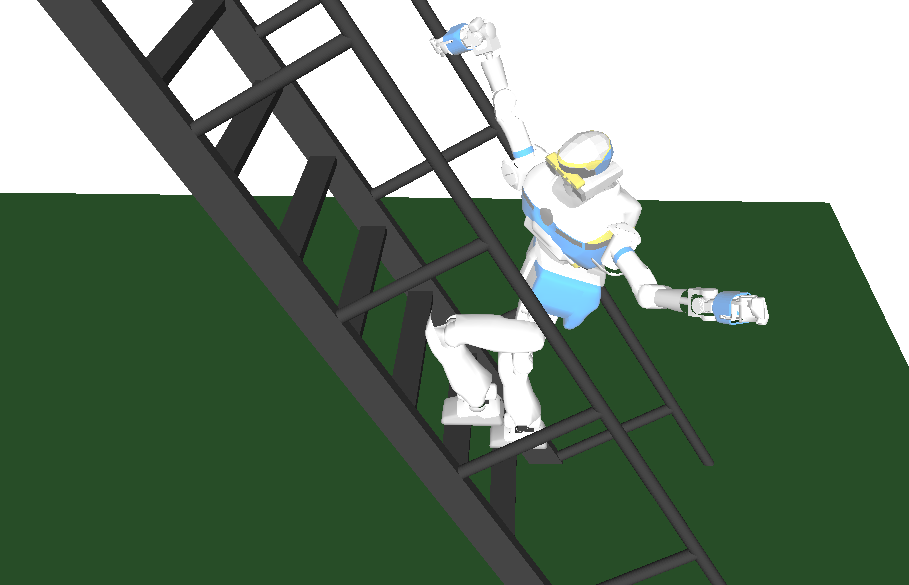
\includegraphics[width=\linewidth]{figure/hrp2_ladder_darpa_40.png}}
%  \fbox{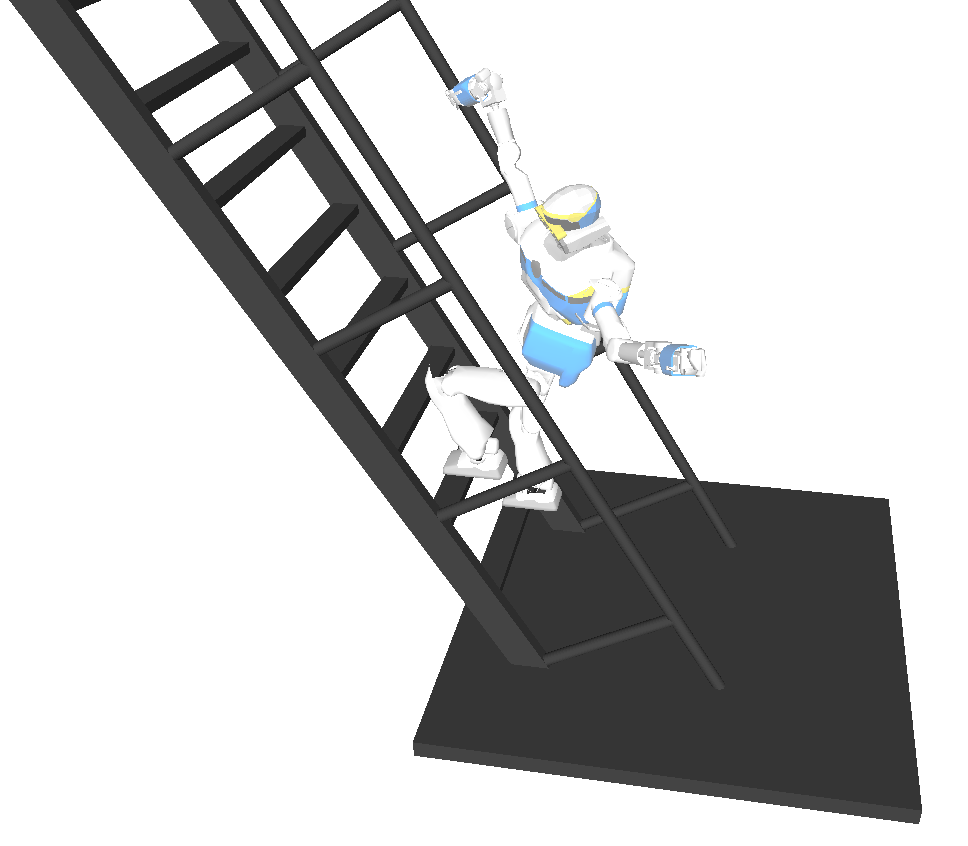
\includegraphics[width=\linewidth]{figure/hrp2_darpa_small.png}}
%  %\caption{HRP2-10 ladder climbing posture}
%  \label{fig:hrp2_darpa}
%\end{subfigure}%
%\begin{subfigure}{.5\textwidth}
%  \centering
%  \setlength\fboxsep{0pt}
%  \setlength\fboxrule{1pt}
%  %\fbox{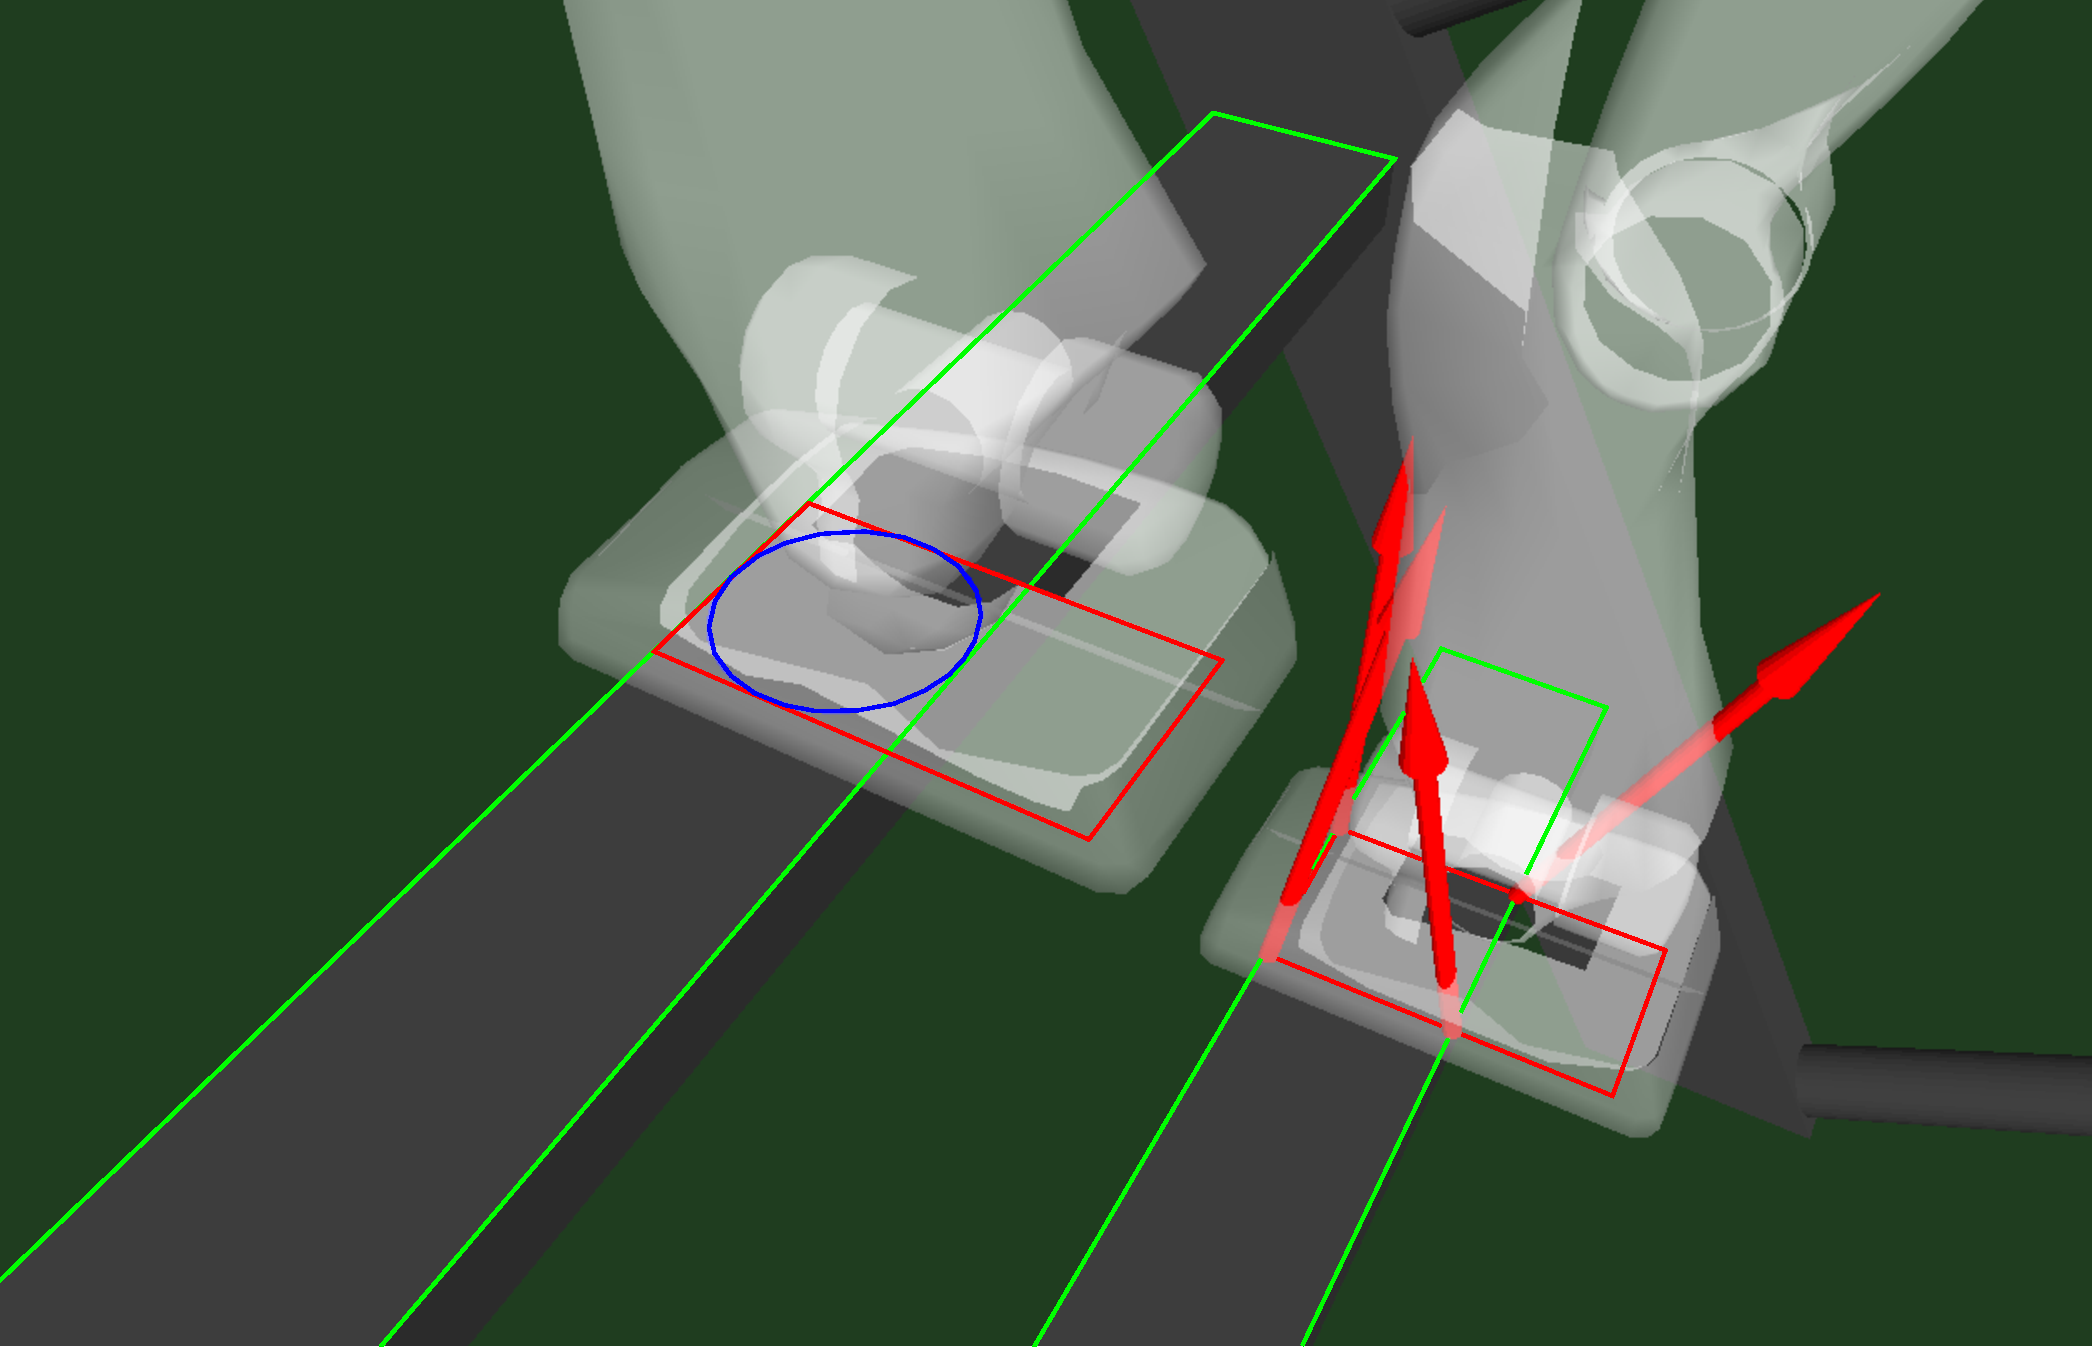
\includegraphics[width=\linewidth]{figure/hrp2_ladder_darpa_zoom.pdf}}
%  %\fbox{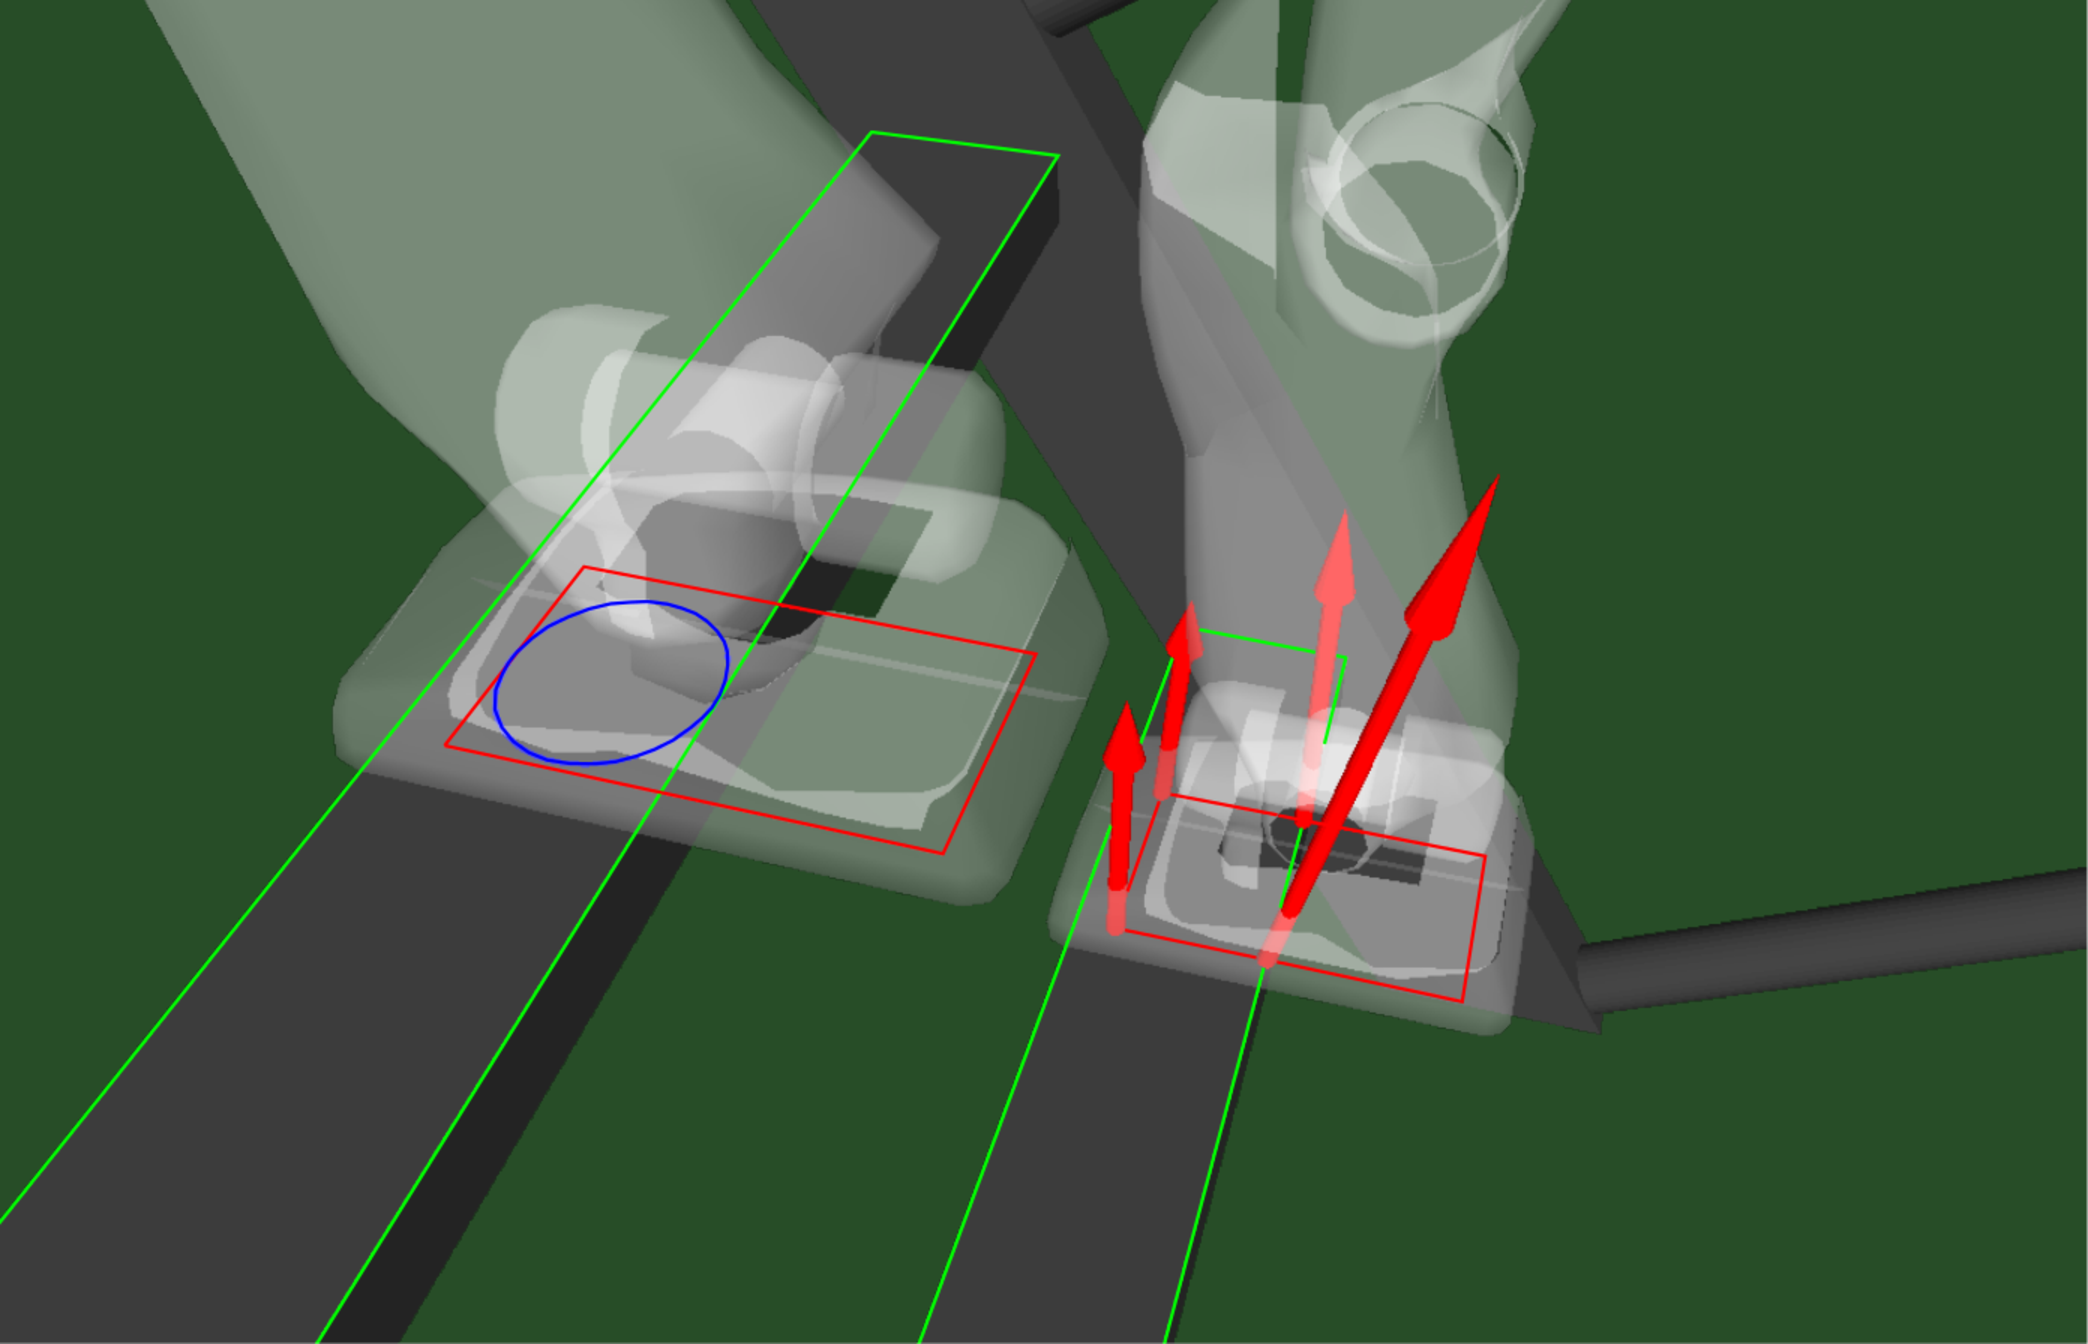
\includegraphics[width=\linewidth]{figure/hrp2_ladder_darpa_40_zoom.pdf}}
%  \fbox{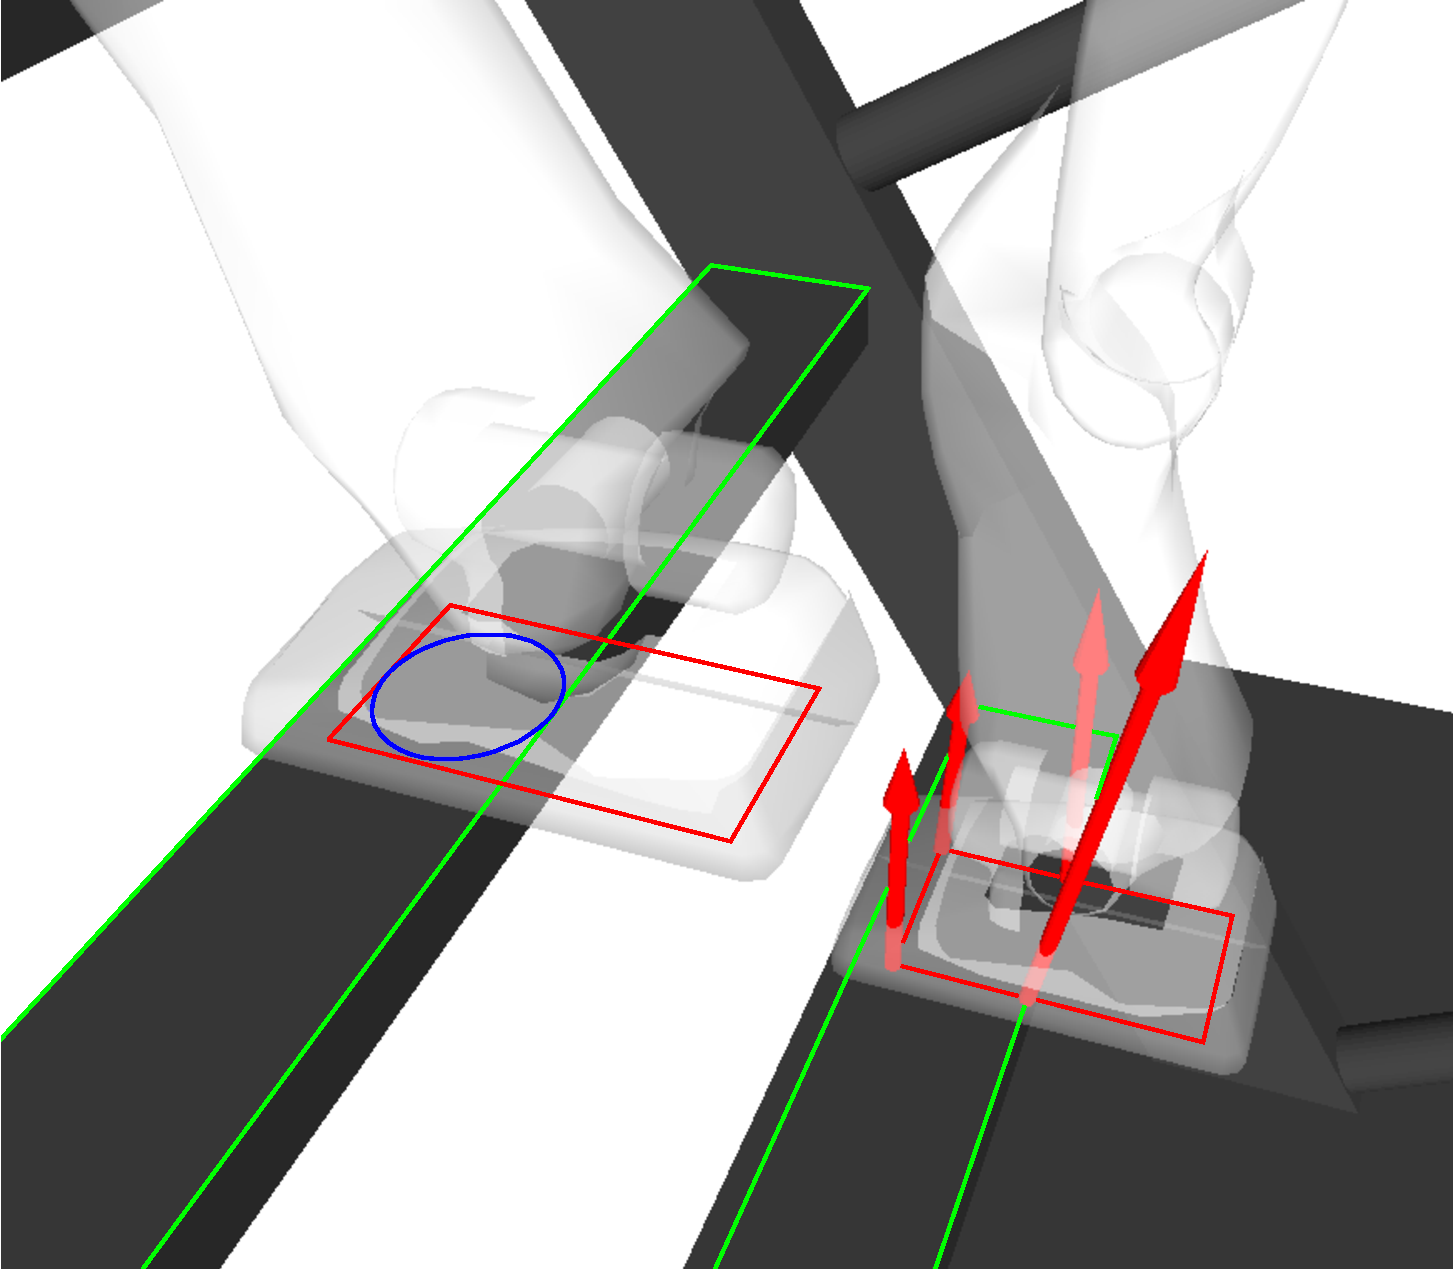
\includegraphics[width=\linewidth]{figure/hrp2_darpa_small_zoom.pdf}}
%  %\caption{Upclose view of the contact areas (green and red: contact polygon, blue: ellipse found in contact area, Red arrows: contact forces resultants)}
%  \label{fig:hrp2_darpa_zoom}
%\end{subfigure}
%\caption{(a)HRP2-10 ladder climbing posture; (b)Upclose view of the contact areas\\(green/red: contact polygons; blue: ellipse found in contact area; red arrows: contact forces resultants)}
%\label{fig:hrp2_darpa_complete}
%\end{figure*}

%\begin{figure}
%\centering
%\begin{subfigure}{.3325\columnwidth}
  %\centering
  %\setlength\fboxsep{0pt}
  %\setlength\fboxrule{1pt}
  %\fbox{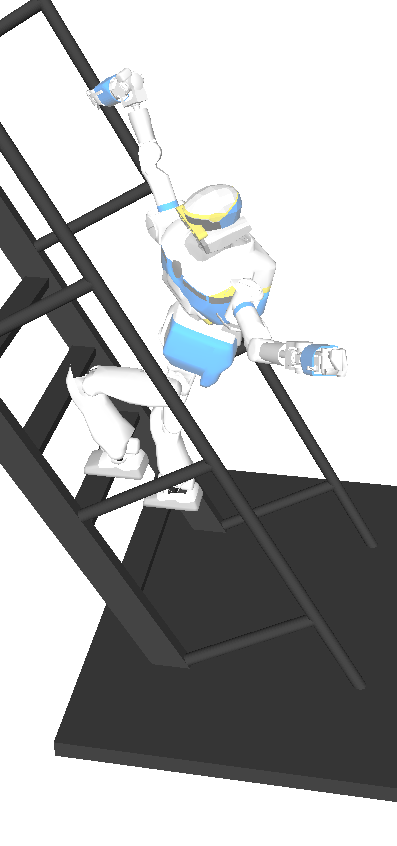
\includegraphics[width=0.95\linewidth]{hrp2_darpa_small_cut.png}}
%\label{fig:hrp2_darpa}
%\end{subfigure}%
%\begin{subfigure}{.6175\columnwidth}
  %\centering
  %\setlength\fboxsep{0pt}
  %\setlength\fboxrule{1pt}
  %\fbox{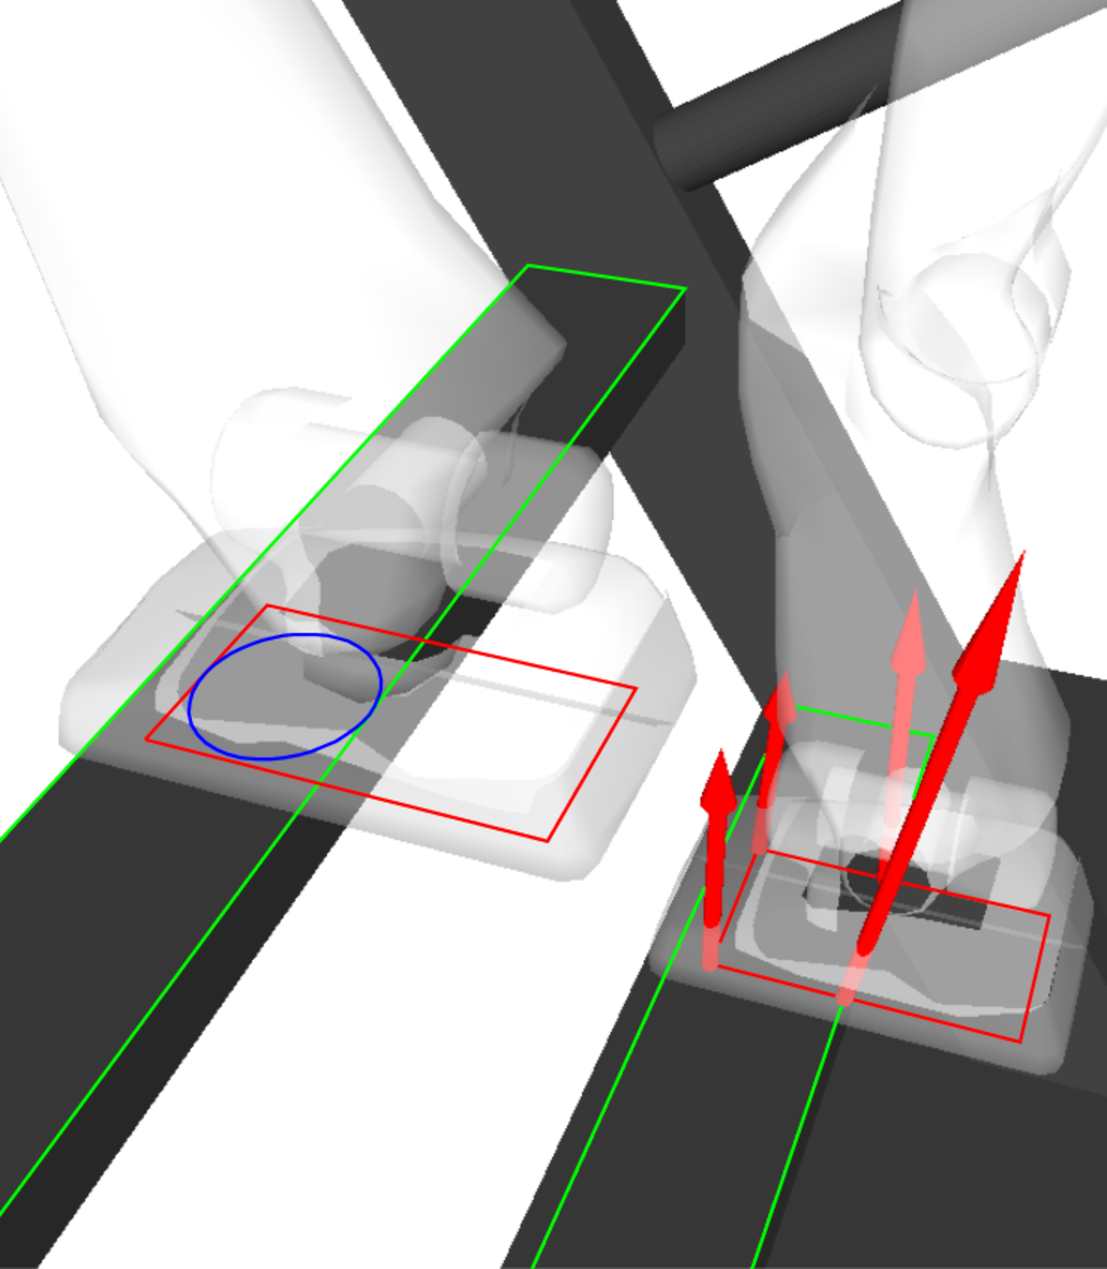
\includegraphics[width=0.95\linewidth]{hrp2_darpa_small_zoom_cut.pdf}}
%\label{fig:hrp2_darpa_zoom}
%\end{subfigure}
%\caption{HRP2 ladder climbing posture and up close view of the contact areas (green/red: contact polygons; blue: contact ellipse; red arrows: contact forces resultants)}
%\label{fig:hrp2_darpa_complete}
%\end{figure}

\begin{figure}[htpb]
  \centering
  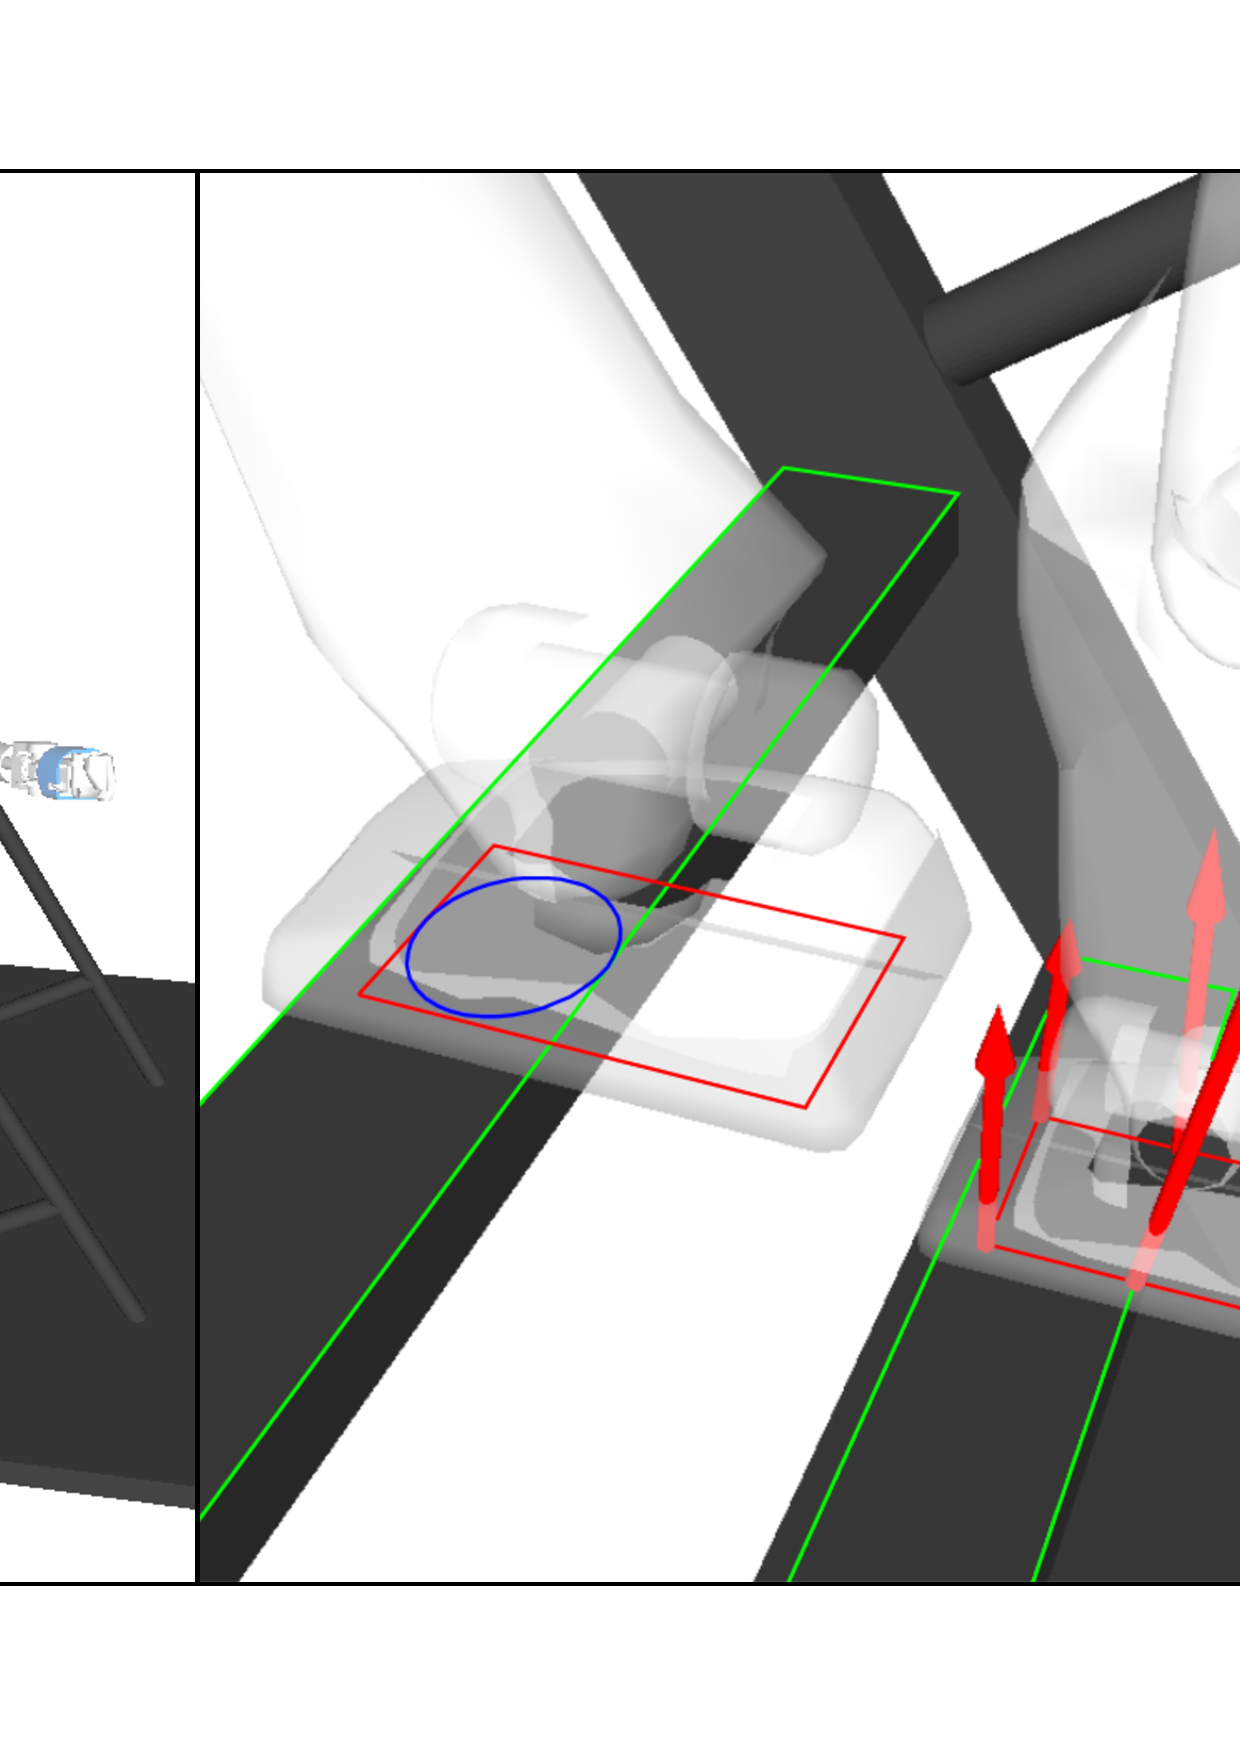
\includegraphics[width=0.8\linewidth]{hrp2_inclined_ladder.pdf}
  \caption{HRP2 ladder climbing posture and up close view of the contact areas (green/red: contact polygons; blue: contact ellipse; red arrows: contact forces resultants)}
\label{fig:hrp2_darpa_complete}
\end{figure}

\begin{figure*}
\centering
\setlength\fboxsep{0pt}
\setlength\fboxrule{1pt}
\fbox{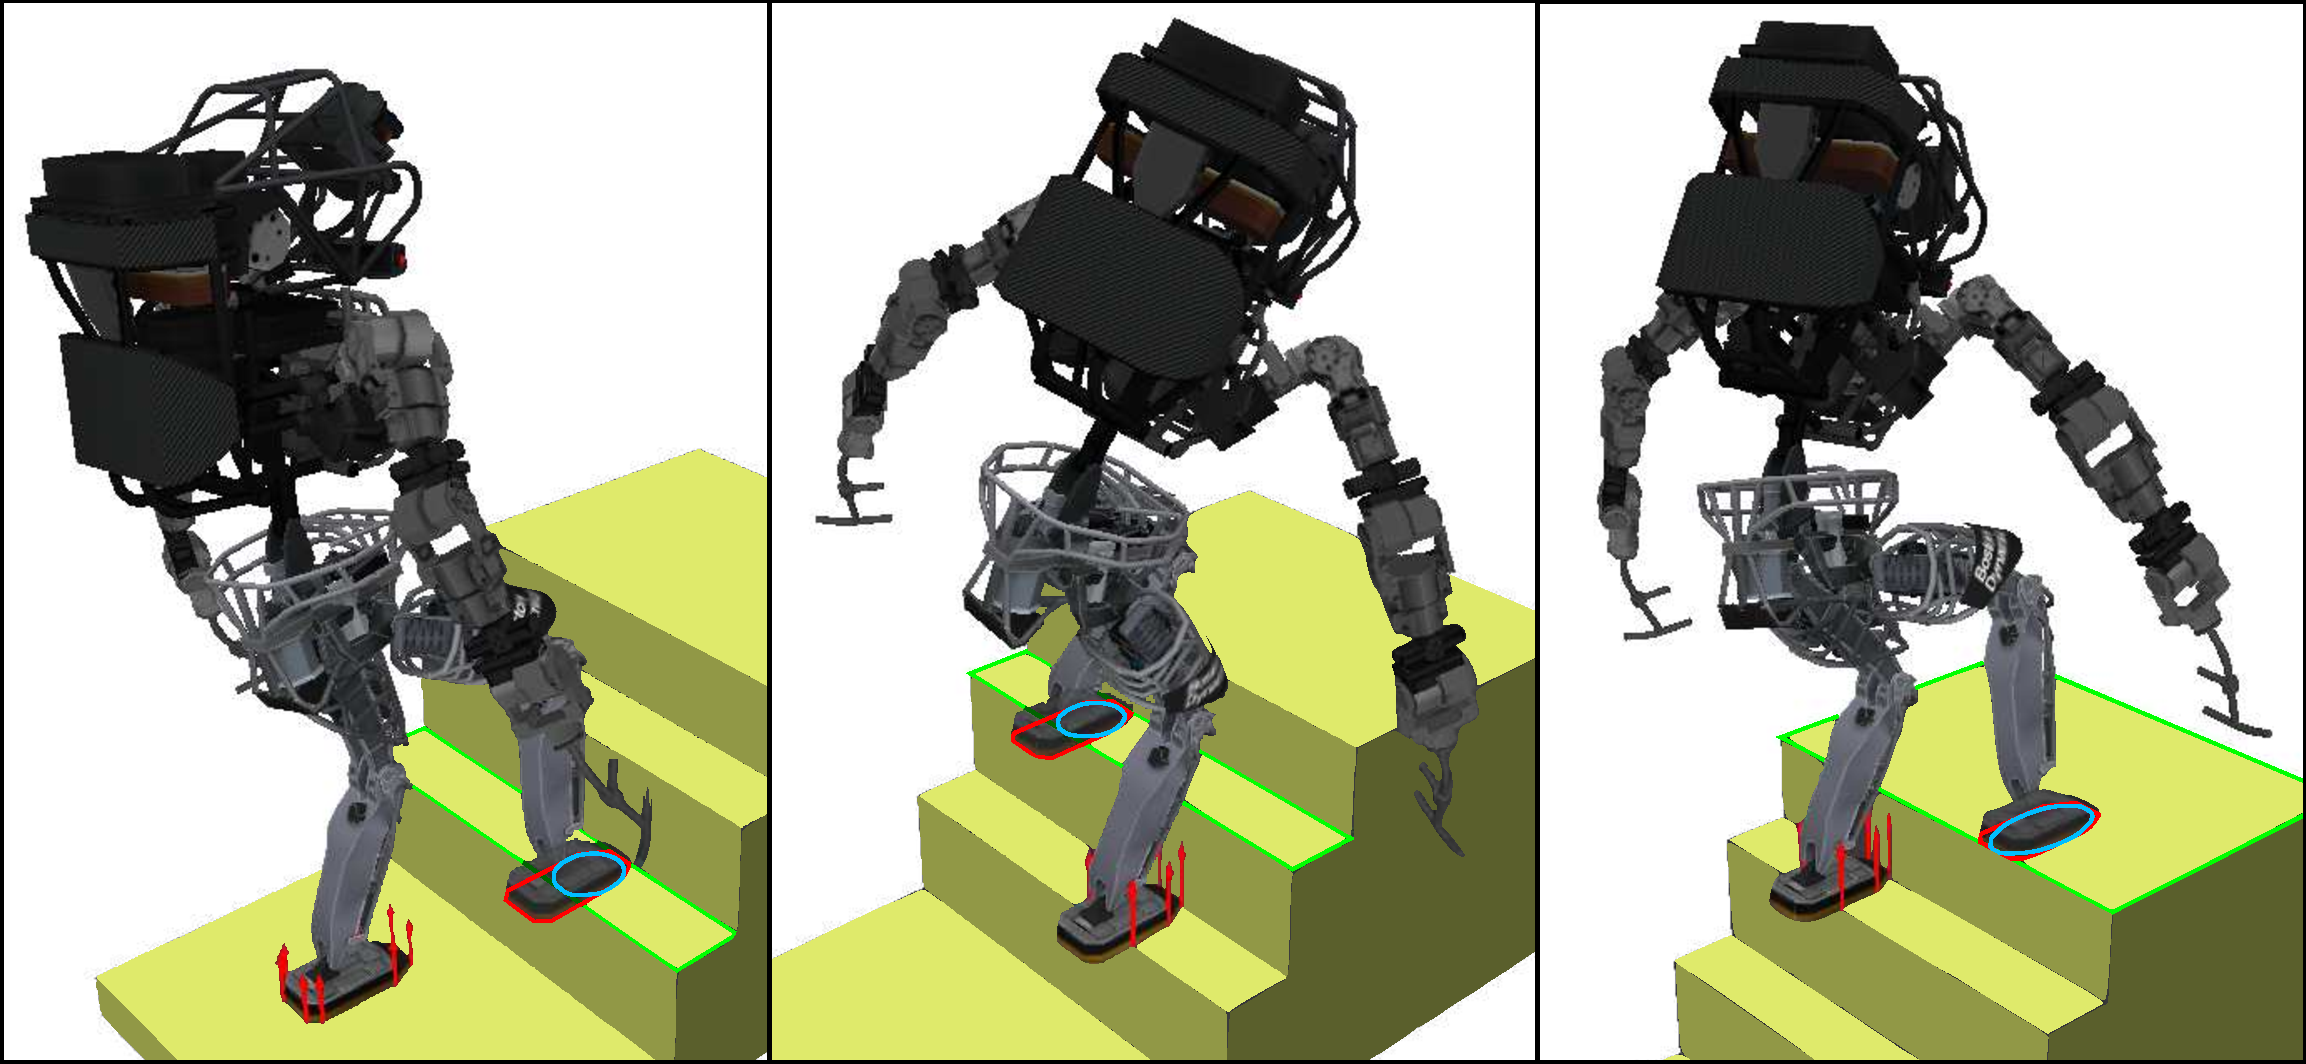
\includegraphics[width=0.95\linewidth]{fixed_atlas_1_2_3_yellow.pdf}}
\caption{Atlas climbing stairs with small steps by maximizing the size of the contact areas\\(green/red: contact polygons; blue: contact ellipse; red arrows: contact forces resultants)}
\label{fig:atlas_SmallStairs}
\end{figure*}



\subsubsection{Vertical ladder climbing}
\label{subsubsec:ladder}

%%%%%%%%%%%%%%%%%%%%%%%%%%%%%%%%%%%%%%%%%%%%%%%%%%%%%%%%%%%%%%%%%%%%%%%
%               SUBSUBSECTION VERTICAL LADDER CLIMBING                %
%%%%%%%%%%%%%%%%%%%%%%%%%%%%%%%%%%%%%%%%%%%%%%%%%%%%%%%%%%%%%%%%%%%%%%%

In the second example, we generate a posture in which the robot climbs a vertical ladder.
In this particular step, the robot is using its right foot and both hands to maintain its stability on top of the first rung of the ladder.
We search a posture that keeps those previous contacts and adds a geometrical contact between the left foot and the second rung of the ladder.
The result of that optimization can be observed on figure~\ref{fig:hrp2_jrl_complete}, with the robot posture on the left and a close-up look at the contact areas on the right.
The difficulty of this situation is that a contact has to be made with a very thin surface of the environment (the ladder rung).
%Usual contact generation method would reduce a lot the span of possible contact positions (by patching the robot's foot with a very small surface or by imposing a set of authorized contact positions).
%Whereas with our method, the contact configuration is found during the optimization process without requiring any extra human work.
The contact chosen by our software includes an ellipse which first axis is the width of the robot's foot and second axis is as thin as the ladder rung.
%One problem to expect is that numerical instability might happen if the surface of the rung is given too thin.
%But that would also happen with full inclusion constraints.
This example also illustrates one limitation of our method: it only considers planar contacts and if one wants to model a purely linear contact another contact model must be used, since our modeling of those singular cases is approximative.
%is the first step of the HRP-2 robot climbing a ladder.
%The two hands are in bilateral contact with the two side bars of the ladder, the left foot is fixed on the ground and is the only part of the robot involved in the stability.
%The right foot is to make a contact with the first rung of the ladder.
%The rungs of the ladder are modeled by rectangles with a 6mm width which approximates the contact line as explained in section~\ref{subsubsec:singular cases}.
%Therefore, the ellipse area maximization takes place in the intersection of the polygons representing the rung and the foot.
%The result of that optimization can be observed on ~\Figref{fig:ladder}{}.
%On the right of the simulation image is shown the disposition of the foot (in green) that is in geometrical non-inclusive contact with a rung (in blue) and the optimal ellipse that has been found.


%From a planning point of view, this particular result is obviously not achievable as the right leg of the robot goes through the ladder, this will be discussed in the next section.
%Yet, the posture is perfectly valid as it respects of the constraints of problem~(\Eqref{eq:PG_chap2}).
%This example illustrates our method in a multi-contact environment with almost linear contacts.
%



\subsubsection{Climbing Stairs}
\label{subsubsec:smallStairs}

%%%%%%%%%%%%%%%%%%%%%%%%%%%%%%%%%%%%%%%%%%%%%%%%%%%%%%%%%%%%%%%%%%%%%%%
%                   SUBSUBSECTION CLIMBING STAIRS                     %
%%%%%%%%%%%%%%%%%%%%%%%%%%%%%%%%%%%%%%%%%%%%%%%%%%%%%%%%%%%%%%%%%%%%%%%

In a third simulation, the ATLAS robot climbs a flight of stairs.
All the steps are too small for the robot to put its entire foot on.
Therefore, it has to make a non-inclusive contact and we propose to maximize the size of the contact area with the ellipse included in it, as explained in Section~\ref{subsubsec:optim-ellipse-area}.
The size of the contact area is limited by the fact that the foot cannot penetrate the wall behind each step.
On~\Figref{fig:atlas_SmallStairs}, we present 3 postures generated in this environment.
On each of those postures, we see that the ellipse's size is maximized until the foot enters in collision with the vertical wall behind each step.
And when possible, like on the last step, the contact area is maximized without collision limitation and the foot is positioned as fully included in the support surface.
We can see here that even when the size of the ellipse is maximized while competing with other nonlinear constraints like collision avoidance, our method still works well and leads us to a satisfactory solution.
It has been used to actually make the robot climb a vertical ladder and presented in~\cite{vaillant:autonomousrobots:2016} and~\cite{vaillant:humanoids:2014}.

%Under each simulation result, an image presents the disposition of the foot (in green) that is in geometrical non-inclusive contact with a step (in blue) and the optimal ellipse that has been found.
%It has to be noted that the green contact surface under a foot of the robot (green rectangle) is actually smaller than the actual foot due to our use of security margin for stability reason when experimenting with real robot and take into account an un-modeled flexibility at the ankle.
%That is why, with the collision avoidance activated between the foot and the next step, it seems that the foot is still far from the limit of the step (blue rectangle).
%Actually the foot is almost in collision with the vertical part of the next step.
%We decided not to present the initial and final steps of this hypothetical movement because they do not bear any interesting aspect as they both consist of the robot standing on a large flat surface.

%\begin{figure*}
%\centering
%\begin{subfigure}{.319\textwidth}
%  \centering
%  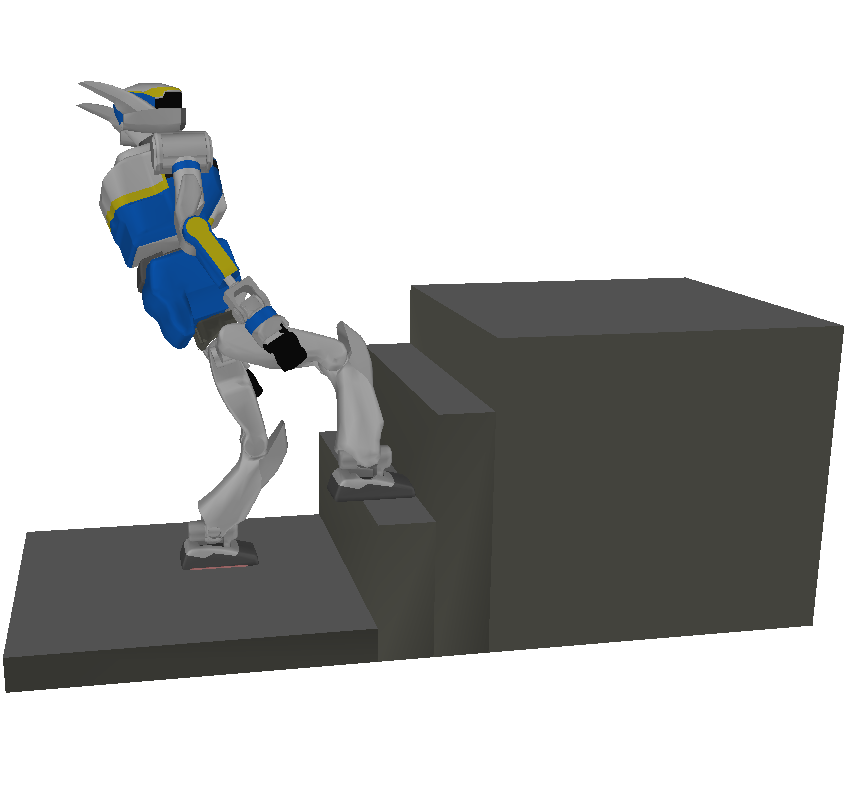
\includegraphics[width=\linewidth]{SmallStairs2.png}
%\end{subfigure}%
%\begin{subfigure}{.3\textwidth}
%  \centering
%  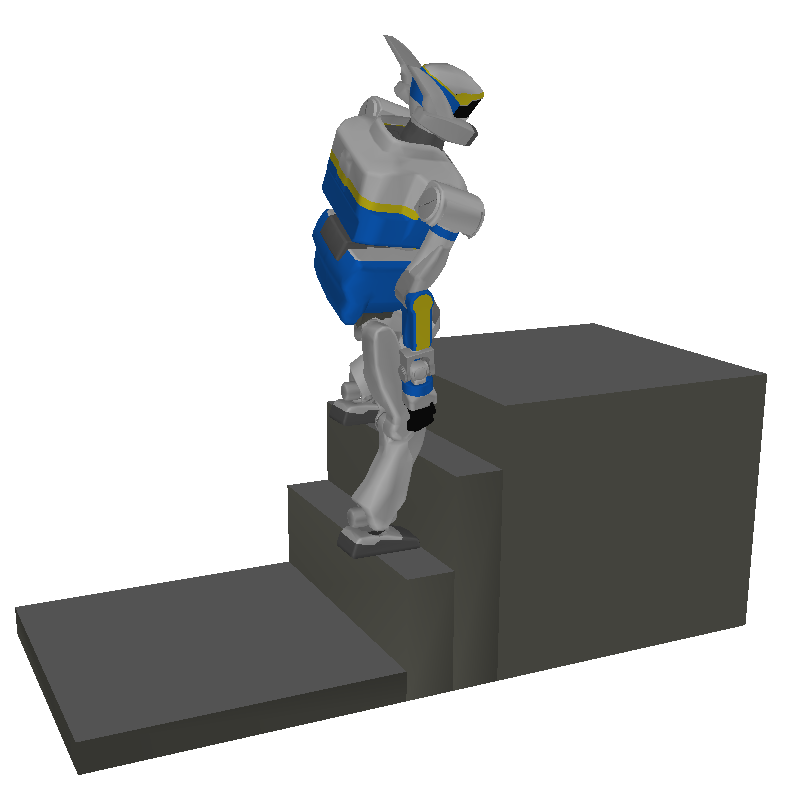
\includegraphics[width=\linewidth]{SmallStairs3.png}
%\end{subfigure}
%\begin{subfigure}{.3\textwidth}
%  \centering
%  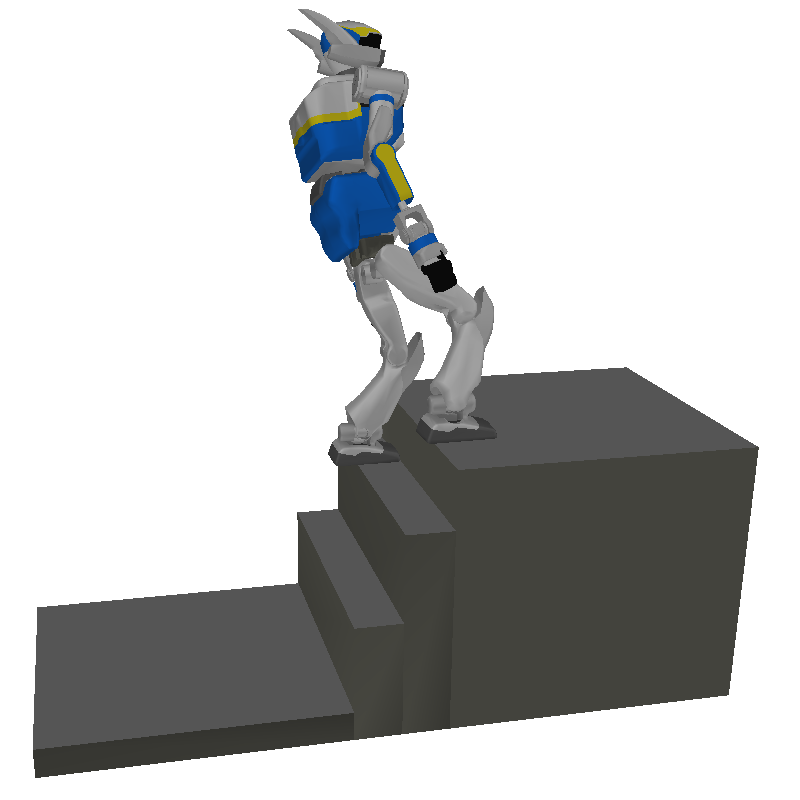
\includegraphics[width=\linewidth]{SmallStairs4.png}
%\end{subfigure}
%\caption{Using non-inclusive contacts for ladder climbing}
%\label{fig:hrp2_SmallStairs}
%\end{figure*}



\subsubsection{Walking along a path made of small objects}
\label{subsubsec:riviere}

%%%%%%%%%%%%%%%%%%%%%%%%%%%%%%%%%%%%%%%%%%%%%%%%%%%%%%%%%%%%%%%%%%%%%%%
%      SUBSUBSECTION WALKING ALONG A PATH MADE OF SMALL OBJECTS       %
%%%%%%%%%%%%%%%%%%%%%%%%%%%%%%%%%%%%%%%%%%%%%%%%%%%%%%%%%%%%%%%%%%%%%%%

In the last simulation, the HRP-2 robot has to cross a gap by making contacts
with small surfaces.
As for the previous simulation, the two objects
with which the feet of the robot will be in contact are too small for making a
complete contact, instead, non-inclusive geometric contacts are found by
maximizing the area of an ellipse that fits in the intersection of the polygons
involved in the contact.
Results are presented in figure~\ref{fig:riviere}.
As we can see, the feet turns slightly, to be more aligned with the support
surfaces, yet they do not become completely aligned with these supports, which would permit to get the biggest ellipse area.
This is due to the fact that a posture cost is competing with the area cost, yielding this compromise.
Under each simulation result, an image presents the disposition of the foot (in green) that is in geometrical non-inclusive contact with a step (in blue) and the optimal ellipse that has been found.
%We decided not to present the initial and final steps of this hypothetical movement because they do not bear any interesting aspect as they both consist of the robot standing on a large flat surface.

\begin{figure*}[!htb]
  \centering
  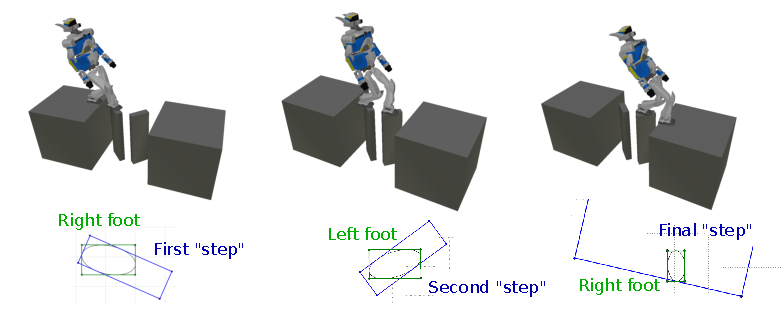
\includegraphics[width=0.95\textwidth]{riviere3steps.pdf}
  \caption{Simulation results for crossing a gap by walking on small items}
\label{fig:riviere}
\end{figure*}



\subsection{Discussion and conclusion}

%%%%%%%%%%%%%%%%%%%%%%%%%%%%%%%%%%%%%%%%%%%%%%%%%%%%%%%%%%%%%%%%%%%%%%%
%          SUBSECTION DISCUSSION AND CONCLUSION                       %
%%%%%%%%%%%%%%%%%%%%%%%%%%%%%%%%%%%%%%%%%%%%%%%%%%%%%%%%%%%%%%%%%%%%%%%

Generating arbitrarily shaped contact areas proved to be doable very simply in an optimization based posture generation module.
We focused on writing constraints that have continuous gradients since the posture generation problem is dominantly smooth.
Hence, our geometric contact model can be useful for other optimization based purposes, for example, control or trajectory optimization, and any gradient-based descent scheme which handles inequalities (e.g.~\cite{escande:icra:2010}).
While we were expecting an increase of computation time due to the addition of new variables in the problem (5 more for a total of 80--100 variables)
we noticed that the timings obtained with this method are sensibly the same that with our previous version of the posture generator with full contact surface inclusion.
Consequently, this method offering a richer contact search (exploration) during planning comes without degrading computation time.
In fact, it truly allows us to substantially reduce the time spent by the user in ad-hoc tuning the shapes of the contact patches, or fixing the contact positions that were previously done by hand.
Also, it is fairly easy to implement and extends multi-contact planning algorithms like the one described in~\cite{escande:ras:2013} to give it richer planning possibilities.
This method extends straightforwardly to point cloud data as far as polygonal convex patches can be extracted.
But one of its limitation is that in its current form, it cannot handle contacts with non-convex surfaces.

%There are several opportunities for future work.
%For example, we could improve the generality of our contact constraint formulation even further to manage linear and punctual contacts without the approximations we currently use.
%Also we could extend our method to allow dealing with non-convex surfaces.
%And finally we would like to apply our method to other fields that use contact generation, like trajectory or control optimization.
%While we were expecting an increase of computation time due to the addition of new variables in the problem (5 more for a total of 80-100 variables), we were surprised by the obtained timings, around $10s$ while a usual posture generation is less than $1s$.
%Part of this increase is obviously due to the fact that we used finite differences to compute the gradients of the new constraints and objectives, and one of the immediate on-going works is to derive and implement efficiently analytical gradients.
%Still, we will also investigate more thoroughly how the new constraints interact with the existing ones to look for potential other causes for this increase.

%Finally, on a planning point of view, ~\Figref{fig:ladder} shows us a new challenge: while the posture found is perfectly correct as the robot is stable, not colliding with its environment and the contacts are where we asked them to be, the posture is obviously difficult to attain, if possible at all.
%We will need to investigate what type of heuristic to use to avoid this kind of results in the middle of a plan.


\section{Torque derivation}
\label{sec:torque_derivation}

%%%%%%%%%%%%%%%%%%%%%%%%%%%%%%%%%%%%%%%%%%%%%%%%%%%%%%%%%%%%%%%%%%%%%%%
%                     SECTION TORQUE DERIVATION                       %
%%%%%%%%%%%%%%%%%%%%%%%%%%%%%%%%%%%%%%%%%%%%%%%%%%%%%%%%%%%%%%%%%%%%%%%

In this section, we present an efficient algorithm to compute the Jacobian matrix of the robot's joint torques with respect to all its articular variables and the variables involved in the expression of the external forces applied to this robot.
The evaluation of the joint torques Jacobian matrix is useful to solve optimization problems in which the torques are involved in the constraints or in the cost function.
The computation of the joint torques Jacobian matrix is done by differentiating algorithm~\ref{alg:IS}.
In most cases, the acceleration of gravity could be replaced by its value on earth $\mathbf{a_c} = \vec{0}$ and $\mathbf{a_f} = g \vec{z}$.
For the sake of generality, we keep it as $\mathbf{a_c}$ and $\mathbf{a_f}$ in the algorithm description, which could be useful if the robot is in a moving vehicle, for example.
We first write algorithm~\ref{alg:IS} in its matrix form (which is more convenient for its derivation).

\begin{algorithm}
  \caption{Inverse Static algorithm on Matrix Form}
\label{alg:ISmatrix}
\begin{algorithmic}
  \For{$i = 0:n_B$}\\
  $f^G_i =
  \begin{bmatrix}
    \mathbf{m}^{G}_i \\ \mathbf{f}^{G}_i
  \end{bmatrix}
  =
  \mathbf{I}^W
  \begin{bmatrix}
    {{}^i\mathbf{R}_W} & \mathbf{0} \\
    -{{}^i\mathbf{R}_W}\widehat{{}^i\mathbf{t}_W} & {{}^i\mathbf{R}_W} \\
  \end{bmatrix}
  \begin{bmatrix}
    \mathbf{a_c} \\ \mathbf{a_f}
  \end{bmatrix}
  -
  \begin{bmatrix}
    {{}^i\mathbf{R}_W} & -{{}^i\mathbf{R}_W}\widehat{{}^i\mathbf{t}_W} \\
    \mathbf{0} & {{}^i\mathbf{R}_W} \\
  \end{bmatrix}
  \begin{bmatrix}
    \mathbf{m}^{ext}_i \\ \mathbf{f}^{ext}_i
  \end{bmatrix}
  $
  \EndFor{}
  \For{$i = n_J-1:0$}
  \State$\tau_i = {f^G_i}^T S_i$
  \If{$pred(i) \neq -1$}
  \State$f^G_{pred(i)} \leftarrow
  \begin{bmatrix}
    \mathbf{m}^{G}_{pred(i)} \\ \mathbf{f}^{G}_{pred(i)}
  \end{bmatrix}
  +
  \begin{bmatrix}
    {\mathbf{R}^{PtS}_i}^T & \widehat{\mathbf{t}^{PtS}_i}{\mathbf{R}^{PtS}_i}^T \\
    \mathbf{0} & {\mathbf{R}^{PtS}_i}^T \\
  \end{bmatrix}
  \begin{bmatrix}
    \mathbf{m}^{G}_i \\ \mathbf{f}^{G}_i
  \end{bmatrix}
  $
  \EndIf{}
  \EndFor{}
\end{algorithmic}
\end{algorithm}

The variables of this algorithm w.r.t. which we need to differentiate it, are the configuration of the robot $q$ and the variables of the external wrenches which can themselves depend on $q$ and some other variables $y$, for example, in the case of a contact with another robot, the application point and value of those forces depend on $q$ and on the configuration of the other robot.
We denote $\dim(q)$ and $\dim(y)$ the dimensions of $q$ and $y$ respectively.
We assume that the derivatives of $m_i^{ext}$ and $f_i^{ext}$: $\frac{\partial m_i^{ext}}{\partial q}$, $\frac{\partial m_i^{ext}}{\partial y}$, $\frac{\partial f_i^{ext}}{\partial q}$, and $\frac{\partial f_i^{ext}}{\partial y}$ are known.

Besides $m_i^{ext}$ and $f_i^{ext}$, all the quantities of the algorithm depend only on $q$.
Therefore, the derivation w.r.t $y$ is trivial and is automatically computed by our final algorithm.
From here we will focus on the derivation w.r.t $q$.

Recall the expression of the Jacobian of a robot's body:
\begin{equation}
  \mathbf{Jac}^W_i =
  \begin{bmatrix}
    \frac{\partial {}^i\mathbf{R}_W}{\partial q_0} & \cdots &
    \frac{\partial {}^i\mathbf{R}_W}{\partial q_j} & \cdots &
    \frac{\partial {}^i\mathbf{R}_W}{\partial q_{dof}} \\
    \frac{\partial {}^i\mathbf{t}_W}{\partial q_0} & \cdots &
    \frac{\partial {}^i\mathbf{t}_W}{\partial q_j} & \cdots &
    \frac{\partial {}^i\mathbf{t}_W}{\partial q_{dof}}
  \end{bmatrix}
=
  \begin{bmatrix}
    \omega_{i,0} & \cdots &
    \omega_{i,j} & \cdots &
    \omega_{i,dof} \\
    v_{i,0} & \cdots &
    v_{i,j} & \cdots &
    v_{i,dof}
  \end{bmatrix}
\end{equation}

Note the following relations that make use of the robot's Jacobian to compute derivatives:
\begin{align}
  \frac{\partial {}^i\mathbf{R}_W \mathbf{u}}{\partial q_j}
  &= {}^i\mathbf{R}_W \mathbf{u} \wedge \omega_{i,j}
  = {}^i\mathbf{R}_W \widehat{\mathbf{u}} \omega_{i,j}
  \\
  \frac{\partial {}^i\mathbf{R}_W {}^i\mathbf{t}_W\wedge \mathbf{u}}{\partial q_j}
  &= {}^i\mathbf{R}_W \mathbf{v}_{i,j} \wedge \mathbf{u}
  + {}^i\mathbf{R}_W \left({}^i\mathbf{t}_W\wedge\mathbf{u}\right) \wedge \omega_{i,j}\\
  &= -{}^i\mathbf{R}_W \widehat{\mathbf{u}} \mathbf{v}_{i,j}
  + {}^i\mathbf{R}_W \widehat{\left(\widehat{{}^i\mathbf{t}_W}\mathbf{u}\right)} \omega_{i,j}
\end{align}

Let's differentiate the first equation of~\ref{alg:ISmatrix} w.r.t $q_j$.

\begin{align}
  A &=
  \begin{bmatrix}
    {{}^i\mathbf{R}_W} & \mathbf{0} \\
    -{{}^i\mathbf{R}_W}\widehat{{}^i\mathbf{t}_W} & {{}^i\mathbf{R}_W} \\
  \end{bmatrix}
  \begin{bmatrix}
    \mathbf{a_c} \\ \mathbf{a_f}
  \end{bmatrix} \\
  B &=
  \begin{bmatrix}
    {{}^i\mathbf{R}_W} & -{{}^i\mathbf{R}_W}\widehat{{}^i\mathbf{t}_W} \\
    \mathbf{0} & {{}^i\mathbf{R}_W} \\
  \end{bmatrix}
  \begin{bmatrix}
    \mathbf{m}^{ext}_i \\ \mathbf{f}^{ext}_i
  \end{bmatrix} \\
  f^G_i &= \mathbf{I}^W A-B\\
  \frac{\partial A}{\partial q_j} &=
  \begin{bmatrix}
    {}^i\mathbf{R}_W \widehat{\bf ac} \omega_{i,j}\\
    -{{}^i\mathbf{R}_W}\widehat{\left(\widehat{{}^i\mathbf{t}_W}{\bf ac} \right)}\omega_{i,j}
    + {{}^i\mathbf{R}_W}\widehat{\bf ac} v_{i,j} + {}^i\mathbf{R}_W \widehat{\bf af} \omega_{i,j}\\
  \end{bmatrix}
  \\
  \frac{\partial B}{\partial q_j} &=
  \begin{bmatrix}
    - {{}^i\mathbf{R}_W}\widehat{\left(\widehat{{}^i\mathbf{t}_W}\bf \mathbf{f}^{ext}_i \right)}\omega_{i,j}
    + {{}^i\mathbf{R}_W}\widehat{\bf \mathbf{f}^{ext}_i} v_{i,j} + {}^i\mathbf{R}_W \widehat{\bf \mathbf{m}^{ext}_i} \omega_{i,j}\\
    {}^i\mathbf{R}_W \widehat{\bf \mathbf{f}^{ext}_i} \omega_{i,j}\\
  \end{bmatrix}
  \\&+
  \begin{bmatrix}
    {{}^i\mathbf{R}_W} & -{{}^i\mathbf{R}_W}\widehat{{}^i\mathbf{t}_W} \\
    \mathbf{0} & {{}^i\mathbf{R}_W} \\
  \end{bmatrix}
  \begin{bmatrix}
    \frac{\partial \mathbf{m}^{ext}_i}{\partial q} \\ \frac{\partial \mathbf{f}^{ext}_i}{\partial q}
  \end{bmatrix}
\end{align}

We rearrange the equations in order to make the jacobian appear.
Putting all the pieces of $\omega$ and $v$ together allows grouping all the j-derivatives to obtain the derivative of $f^G_i$ with a single equation.

\begin{align}
  \bf M &=
  \begin{bmatrix}
    {}^i\mathbf{R}_W \widehat{\bf ac}  & 0\\
    -{{}^i\mathbf{R}_W}\widehat{\left(\widehat{{}^i\mathbf{t}_W}\bf ac \right)}
    + {}^i\mathbf{R}_W \widehat{\bf af}  & {{}^i\mathbf{R}_W}\widehat{\bf ac} \\
  \end{bmatrix}
  \\
  \bf N &=
  \begin{bmatrix}
    - {{}^i\mathbf{R}_W}\widehat{\left(\widehat{{}^i\mathbf{t}_W}\bf \mathbf{f}^{ext}_i \right)} + {}^i\mathbf{R}_W \widehat{\bf \mathbf{m}^{ext}_i} & {{}^i\mathbf{R}_W}\widehat{\bf \mathbf{f}^{ext}_i} \\
    {}^i\mathbf{R}_W \widehat{\bf \mathbf{f}^{ext}_i} & 0\\
  \end{bmatrix}
  \\
  \frac{\partial f^G_i}{\partial q} &= (\mathbf{I}^W \mathbf{M} - \mathbf{N})\mathbf{Jac}^W_i
  +
  \begin{bmatrix}
    {{}^i\mathbf{R}_W} & -{{}^i\mathbf{R}_W}\widehat{{}^i\mathbf{t}_W} \\
    \mathbf{0} & {{}^i\mathbf{R}_W} \\
  \end{bmatrix}
  \begin{bmatrix}
    \frac{\partial \mathbf{m}^{ext}_i}{\partial q} \\ \frac{\partial \mathbf{f}^{ext}_i}{\partial q}
  \end{bmatrix}
\end{align}

The derivation of the second equation is obvious:

\begin{align}
  \tau_i &= {f^G_i}^T S_i \\
  \frac{\partial \tau_i}{\partial q} &= S_i^T \frac{\partial f^G_i}{\partial q} \\
\end{align}

Note the following relations:
\begin{align}
  \frac{\partial {\mathbf{R}_i^J}^T \mathbf{u}}{\partial q_j}
  &= - S^R_{i,j} \wedge ({\mathbf{R}_i^J}^T \mathbf{u})
  = \widehat{({\mathbf{R}_i^J}^T \mathbf{u})} S^R_{i,j}
  \\
  \frac{\partial\mathbf{t}^J_i\wedge {\mathbf{R}_i^J}^T  \mathbf{u}}{\partial q_j}
  &= S^t_{i,j} \wedge \left({\mathbf{R}_i^J}^T \mathbf{u}\right)
  - \mathbf{t}^J_i \wedge \left( S^R_{i,j} \wedge \left({\mathbf{R}_i^J}^T \mathbf{u}\right)\right) \\
  &= -\widehat{({\mathbf{R}_i^J}^T \mathbf{u})} S^t_{i,j}
  + \left(\left({\mathbf{R}_i^J}^T \mathbf{u}\right) \cdot {\mathbf{t}^J_i}^T
  - \left( {({\mathbf{R}_i^J}^T \mathbf{u})}^T \cdot \mathbf{t}^J_i\right) \mathbf{I}_3\right)S_{i,j}^R\\
\end{align}

The last equation's derivation goes as follows:

\begin{align}
  f^G_{pred(i)} & \leftarrow f^G_{pred(i)} +
  \begin{bmatrix}
    {\mathbf{R}^{PtS}_i}^T & \widehat{\mathbf{t}^{PtS}_i}{\mathbf{R}^{PtS}_i}^T \\
    \mathbf{0} & {\mathbf{R}^{PtS}_i}^T \\
  \end{bmatrix}
  \begin{bmatrix}
    \mathbf{m}^{G}_i \\ \mathbf{f}^{G}_i
  \end{bmatrix}
  \\
  & =f^G_{pred(i)} + \begin{bmatrix}
    {\mathbf{R}^{x}_i}^T & \widehat{\mathbf{t}^{x}_i}{\mathbf{R}^{x}_i}^T \\
    \mathbf{0} & {\mathbf{R}^{x}_i}^T \\
  \end{bmatrix}
  \begin{bmatrix}
    {\mathbf{R}^{J}_i}^T & \widehat{\mathbf{t}^{J}_i}{\mathbf{R}^{J}_i}^T \\
    \mathbf{0} & {\mathbf{R}^{J}_i}^T \\
  \end{bmatrix}
  \begin{bmatrix}
    \mathbf{m}^{G}_i \\ \mathbf{f}^{G}_i
  \end{bmatrix}
  \\
\end{align}

We define $K_i$ as:
\begin{equation}
  K_i =
  \begin{bmatrix}
    \widehat{({\mathbf{R}_i^J}^T \mathbf{m}^{G}_i)}
    + \left({\mathbf{R}_i^J}^T \mathbf{f}^{G}_i\right) \cdot {\mathbf{t}^J_i}^T
    - \left( {({\mathbf{R}_i^J}^T \mathbf{f}^{G}_i)}^T \cdot \mathbf{t}^J_i\right) \mathbf{I}_3
    & -\widehat{({\mathbf{R}_i^J}^T \mathbf{f}^{G}_i)} \\
    \widehat{({\mathbf{R}_i^J}^T \mathbf{f}^{G}_i)} & 0
  \end{bmatrix}
\end{equation}

\begin{equation}
    \frac{\partial f^G_{pred(i)}}{\partial q} \leftarrow \frac{\partial f^G_{pred(i)}}{\partial q} -
  \begin{bmatrix}
    {\mathbf{R}^{x}_i}^T & \widehat{\mathbf{t}^{x}_i}{\mathbf{R}^{x}_i}^T \\
    \mathbf{0} & {\mathbf{R}^{x}_i}^T \\
  \end{bmatrix}
  K_i \mathbf{S_i}
\end{equation}

In the following algorithm, we use the following notation $x$ to combine the variables $q$ and $y$:
\begin{equation}
  x = \begin{bmatrix}
    q & y
  \end{bmatrix}
\end{equation}

\begin{equation}
  \frac{\partial f_{ext}}{\partial x} =
  \begin{bmatrix}
    \frac{\partial \mathbf{m}^{ext}_i}{\partial q} & \frac{\partial \mathbf{m}^{ext}_i}{\partial y}
    \\
    \frac{\partial \mathbf{f}^{ext}_i}{\partial q} & \frac{\partial \mathbf{f}^{ext}_i}{\partial y}
  \end{bmatrix}
\end{equation}


The entire algorithm for calculating the torque jacobian is presented in Algorithm~\ref{alg:TJC}.

\begin{algorithm}[H]
\caption{Torque Jacobian Calculation}
\label{alg:TJC}
\begin{algorithmic}
  \State{Compute the Jacobian of generalized forces}
  \For{$i = 0:n_B$}
  \State$f^G_i =
  \mathbf{I}^W
  \begin{bmatrix}
    {{}^i\mathbf{R}_W} & \mathbf{0} \\
    -{{}^i\mathbf{R}_W}\widehat{{}^i\mathbf{t}_W} & {{}^i\mathbf{R}_W} \\
  \end{bmatrix}
  \begin{bmatrix}
    \mathbf{a_c} \\ \mathbf{a_f}
  \end{bmatrix}
  -
  \begin{bmatrix}
    {{}^i\mathbf{R}_W} & -{{}^i\mathbf{R}_W}\widehat{{}^i\mathbf{t}_W} \\
    \mathbf{0} & {{}^i\mathbf{R}_W} \\
  \end{bmatrix}
  \begin{bmatrix}
    \mathbf{m}^{ext}_i \\ \mathbf{f}^{ext}_i
  \end{bmatrix}
  $
  \State$\bf M =
    \begin{bmatrix}
    {}^i\mathbf{R}_W \widehat{\bf ac}  & 0\\
    -{{}^i\mathbf{R}_W}\widehat{\left(\widehat{{}^i\mathbf{t}_W}\bf ac \right)}
    + {}^i\mathbf{R}_W \widehat{\bf af}  & {{}^i\mathbf{R}_W}\widehat{\bf ac} \\
    \end{bmatrix}
    $
  \State$\bf N =
  \begin{bmatrix}
    - {{}^i\mathbf{R}_W}\widehat{\left(\widehat{{}^i\mathbf{t}_W}\bf \mathbf{f}^{ext}_i \right)}
    + {}^i\mathbf{R}_W \widehat{\bf \mathbf{m}^{ext}_i}
    & {{}^i\mathbf{R}_W}\widehat{\bf \mathbf{f}^{ext}_i} \\
    {}^i\mathbf{R}_W \widehat{\bf \mathbf{f}^{ext}_i} & 0\\
  \end{bmatrix}
  $
  \State$
  \frac{\partial f^G_i}{\partial x} = (\mathbf{I}^W \mathbf{M} - \mathbf{N})\begin{bmatrix}
      \mathbf{Jac_i^W} & \mathbf{0}_{6\times \dim(y)}
        \end{bmatrix}
  +
  \begin{bmatrix}
    {{}^i\mathbf{R}_W} & -{{}^i\mathbf{R}_W}\widehat{{}^i\mathbf{t}_W} \\
    \mathbf{0} & {{}^i\mathbf{R}_W} \\
  \end{bmatrix}
  \frac{\partial f_{ext}}{\partial x}
  $
  \EndFor{}
  \State{Compute the Jacobian of torques}
  \For{$i = n_J-1:0$}
  \State$\frac{\partial \tau_i}{\partial x} =
  \begin{bmatrix}
    \mathbf{S_i} & \mathbf{0}_{6\times \dim(y)}
  \end{bmatrix}^T \frac{\partial f^G_i}{\partial x}$
  \If{$pred(i) \neq -1$}
  \State$\mathbf{K} =
  \begin{bmatrix}
    \widehat{({\mathbf{R}_i^J}^T \mathbf{m}^{G}_i)}
    + \left({\mathbf{R}_i^J}^T \mathbf{f}^{G}_i\right) \cdot {\mathbf{t}^J_i}^T
    - \left( {({\mathbf{R}_i^J}^T \mathbf{f}^{G}_i)}^T \cdot \mathbf{t}^J_i\right) \mathbf{I}_3
    & -\widehat{({\mathbf{R}_i^J}^T \mathbf{f}^{G}_i)} \\
    \widehat{({\mathbf{R}_i^J}^T \mathbf{f}^{G}_i)} & 0
  \end{bmatrix}$
  \State$f^G_{pred(i)} \leftarrow f^G_{pred(i)} + {\mathbf{X}^{PtS}_i(q)}^{-*} f^G_i$
  \State$\frac{\partial f^G_{pred(i)}}{\partial x} \leftarrow \frac{\partial f^G_{pred(i)}}{\partial x} -
  \begin{bmatrix}
    {\mathbf{R}^{x}_i}^T & \widehat{\mathbf{t}^{x}_i}{\mathbf{R}^{x}_i}^T \\
    \mathbf{0} & {\mathbf{R}^{x}_i}^T \\
  \end{bmatrix}
  \mathbf{K} \cdot \begin{bmatrix}
    \mathbf{S_i} & \mathbf{0}_{6\times \dim(y)}
  \end{bmatrix}$
  \EndIf{}
  \EndFor{}
\end{algorithmic}
\end{algorithm}

This algorithm efficiently computes the exact joint torques Jacobian for a robotic system subject to any type of external forces.

\newpage
\section{On the use of lifted variables for Robotics Posture Generation}
\label{sec:liftedVariables}

%%%%%%%%%%%%%%%%%%%%%%%%%%%%%%%%%%%%%%%%%%%%%%%%%%%%%%%%%%%%%%%%%%%%%%%%%%%
% SECTION ON THE USE OF LIFTED VARIABLES FOR ROBOTICS POSTURE GENERATION  %
%%%%%%%%%%%%%%%%%%%%%%%%%%%%%%%%%%%%%%%%%%%%%%%%%%%%%%%%%%%%%%%%%%%%%%%%%%%

The goal of this thesis is, on the one hand, to enable writing more complex and various problems in simpler ways by improving the formulation of posture generation problems, and on the other hand, to improve and adapt the resolution methods for those problems.
This section focuses on the latter issue.
We formulate posture generation problems in an optimization friendly way in order to solve them using nonlinear constrained optimization algorithms.
In this section, we investigated the usage of the lifted optimization method presented in~\cite{Albersmeyer:2010:LNM:1958447.1958472} to the posture generation problems.
In fact, the authors suggested that their method would be suitable for inverse kinematic problems.

The idea of lifting optimization is to consider a complex equation $F(q) = 0$ and decompose it into simpler functions $\{f_1, f_2, \ldots, f_m\}$ that all depend only on the original variable $q$ and on the output of functions of lower index eq.~(\ref{eq:simplerFunctions}) that are replaced by additional variables $\{w_1, w_2, \ldots, w_m\}$, that are called the `lifted variables'.

\begin{equation}
\label{eq:simplerFunctions}
  w_i = f_i(q, w_1, w_2, \ldots,w_{i-1}),\ \forall i\in[1,\ldots, m]
\end{equation}

Such that they can be used in a chain to recompose $F$:

\begin{align}
  F(q) &= f_F\left(q, w_1, w_2, \ldots, w_m\right)\\
       &= f_F\left(q, f_1(q), f_2(q,w_1), f_3(q,w_1,w_2), \ldots, f_m(q, w_1, \ldots, w_m-1)\right) \\
       &= f_F\left(q, f_1(q), f_2(q,f_1(q)), f_3(q,f_1(q),f_2(q,f_1(q))), \ldots, f_m(q, \ldots, f_{m-1}(q,\cdots))\right)
\end{align}

With this formulation and the additional lifted variables $w_i,\ i\in[1,\ldots, m]$, the problem $F(q) = 0$ can be rewritten as the following lifted problem:

\begin{equation}
\label{eq:lifted_variables}
  G(q,w) =
  \begin{pmatrix}
  f_1(q) - w_1 \\
  f_2(q,w_1) - w_2 \\
  f_3(q,w_1,w_2) - w_3 \\
  \vdots \\
  f_m(q,w_1,\ldots, w_{m-1}) - w_m \\
  f_F(q,w_1,\ldots, w_{m-1}, w_m)
  \end{pmatrix}
  =0
\end{equation}

This modified formulation can be used for any function of our optimization problem to reduce the complexity of individual equations at the cost of adding extra variables and constraints.
By reducing the complexity of the functions, which often results in reducing their polynomial degree, we ought to improve the quality of their quadratic approximations, which should lead to better convergence properties of the Newton scheme.

%The reason for expecting this approach to yield good results is that during the optimization process, at each step, a quadratic approximation of the function $F$ is used to compute the next iterate.
%If $F$ is a complicated function, the quadratic approximation may be quite far from $F$ and simpler functions may have better quadratic approximations, which should lead to better convergence properties of the Newton scheme.

One obvious drawback of this approach for solving nonlinear problems is the increased size of the linearized problem to solve at each iteration of the optimization.
Fortunately,~\cite{Albersmeyer:2010:LNM:1958447.1958472} proposes an algorithmic trick leveraging the triangularity of the Jacobian of $G(q,w)$ to condense the lifted problem into a problem of the same size as the original one.
Thus, the resolution of each iteration should take approximately the same time as with the original problem.

The lifted variable approach is known to be superior to the non-lifted one in the problem of shooting methods for boundary value problems~\cite{osborne:1969:shooting}.
With good intuition, the authors of~\cite{Albersmeyer:2010:LNM:1958447.1958472} state that the lifting idea could be directly transferred in the context of kinematic chains found in robotics.
Indeed, as we state in Section~\ref{sec:forward_kinematics}, the equation that governs the transformation of a robot's end effector on body $i$, ${}^i X_W(q)$ is constructed iteratively and seems to be a good candidate for lifting.
If we consider a single chain robot with $m$ bodies, such that $\kappa (m) = \{0, 1, 2, \ldots m\}$ the ${}^m X_W(q) = X_\text{goal}$ can straightforwardly be lifted as follows:

\begin{equation}
\label{eq:robot_lift}
  G(q,w) =
  \begin{pmatrix}
  {}^1 X_W(q) - w_1 \\
  {}^2 X_1(q)\cdot w_1 - w_2\\
  {}^3 X_2(q)\cdot w_2 - w_3 \\
  \vdots \\
  {}^m X_{m-1}(q)\cdot w_{m-1} - w_{m-1} \\
  w_{m-1} - X_\text{goal}
  \end{pmatrix}
  =0
\end{equation}

The transformation of a body is used in almost all the constraints and cost functions of posture generation problems, thus, we can use this lifting approach in most functions of our problems.
This formulation can be generalized to more complex robots by considering/lifting only the bodies in the direct chain from the base to the end effector.

\subsection{Lifting Algorithm}
\label{subsec:LiftingAlgorithm}

In order to explore the capabilities of optimization on lifted problems, we developed and studied several lifting approaches based on different lifting criterion.
A lifting criterion is a criterion that should be satisfied as best as possible by all the functions present at the end of the lifting process.
For example, the degree of a polynomial can be a used, one could require that all the functions are polynomials of at most degree $m$.
In~\ref{eq:robot_lift}, we lifted based one the criterion that each function should only contain a single joint transformation.

Let us consider an example with a simple planar 2 axis robot, with 2 successive links of length 1 attached by revolute joints.
Its articular variables are denoted $q = (q_1, q_2)$ and the expression of the end-effector's (EE) position is the following:
\begin{equation}
  \left(\begin{array}{c}
    \cos\!\left(q_{1}\right) + \cos\!\left(q_{1}\right)\, \cos\!\left(q_{2}\right) - \sin\!\left(q_{1}\right)\, \sin\!\left(q_{2}\right)\\
    \sin\!\left(q_{1}\right) + \cos\!\left(q_{1}\right)\, \sin\!\left(q_{2}\right) + \cos\!\left(q_{2}\right)\, \sin\!\left(q_{1}\right)
  \end{array}\right)
  =
  \left(\begin{array}{c}
    \text{EE}_{x}(q)\\
    \text{EE}_{y}(q)
  \end{array}\right)
\label{eq:direct_position}
\end{equation}

Those equations are polynomials in the variables $\cos(q_1)$, $\sin(q_1)$, $\cos(q_2)$, $\sin(q_2)$.
Furthermore, they are polynomials of degree $1$ in each of those variables separately.
This observation extends to the case of any robot composed of the joints presented in Section~\ref{sec:joints_formulations} and that does not contain kinematic loops (kinematic loops are not considered in this thesis).
The operators `addition', `subtraction', `multiplication', `sinus' and `cosinus' are enough to describe the kinematics of a robot.

We developed a generic algorithm which allows to automatically lift symbolic functions, and in particular, polynomials of trigonometric functions, based on a given criterion.
To do so, we use symbolic variables.
A symbolic equation can be seen as a graph of atomic operations (addition, multiplication, and other functions), which can, in turn, be explored and truncated at appropriate places where we insert additional variables.
Figure~\ref{fig:graph_direct} presents the graph of atomic operations for equation~\Eqref{eq:direct_position}, where the green circles represent the original variables, the yellow ones represent the lifted variables, the pink ones represent the atomic operations and the red circles represent the final atomic operations that lead to the end effector equations.
\begin{figure}
  \centering
  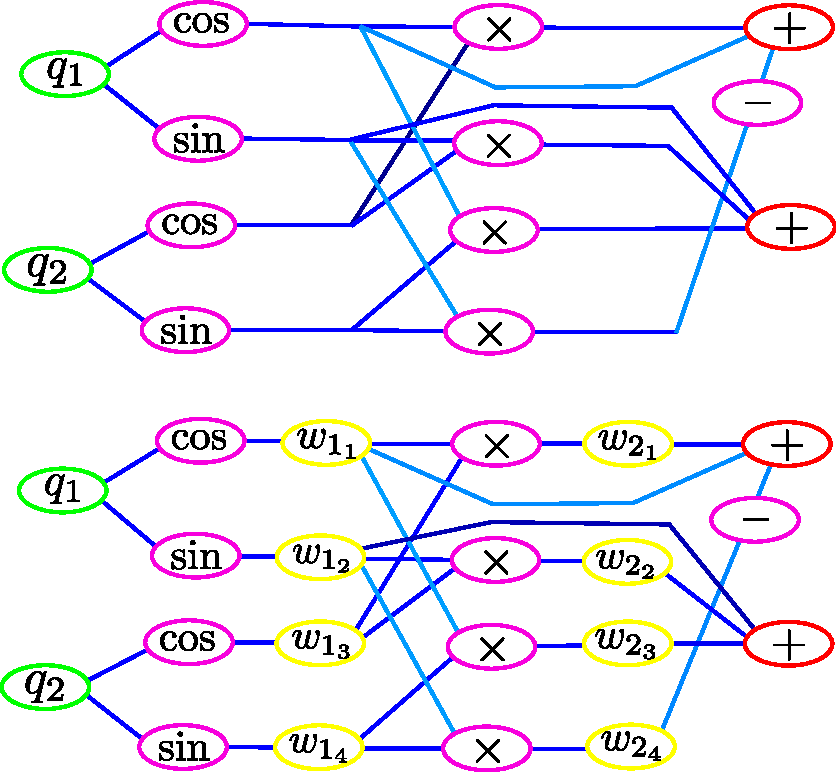
\includegraphics[width=0.65\textwidth]{graphDirectLiftedEEPos.pdf}
  \caption{Computation graph for end effector position of a 2 axis planar robotic arm. Top: Direct equations. Bottom: Lifted equations. Green circles represent the original variables, yellow the lifted ones, pink represent intermediary operations and red represent the final operation for the end effector equations}
\label{fig:graph_direct}
\end{figure}

To lift a set of equations, we explore the graph from left to right.
At each node of the graph, we consider the sub-graph that lies on its left.
If this sub-graph violates our criterion, a lifting variable is added and replaces the sub-graph.
Then we iterate this process on the remaining graph until it does not violate the criterion.
Given that the equations to solve are polynomials in terms of the trigonometric functions, we decided to lift them based on a criterion of maximum degree of the lifted polynomials.
We define the degree function as the degree of a polynomial with the specificity that trigonometric functions are considered to be polynomials of infinite degree (and thus are always lifted, no matter the maximum degree criterion).
We also consider the option of eliminating or not the trigonometric functions.
By eliminating the trigonometric functions, we mean that we reformulate the problem so that, given a variable $x$ that appears in our equations in the forms $\cos(x)$ and/or $\sin(x)$, we introduce 2 new variables $s_x$ and $c_x$; replace all the occurrences of $\cos(x)$ by $c_x$ and all the occurrences of $\sin(x)$ by $s_x$, and to ensure the equivalence of the two formulations, we add the equation ${c_x}^2 + {s_x}^2=1$ to our problem.

For example, lifting the set of equation~\Eqref{eq:direct_position} with a maximum degree of 2 and without eliminating the trigonometric functions gives the following system, with all the $w_{i_j}$ being the additional lifted variables:
\begin{equation}
  \begin{array}{c}
  \textbf{Lifted Equations}\\
  \left(
    \begin{array}{c}
      \cos(q_1) = w_{1_1}\\
      \sin(q_1) = w_{1_2}\\
      \cos(q_2) = w_{1_3}\\
      \sin(q_2) = w_{1_4}\\
      w_{1_1}.w_{1_3} = w_{2_1}\\
      w_{1_2}.w_{1_3} = w_{2_2}\\
      w_{1_1}.w_{1_4} = w_{2_3}\\
      w_{1_2}.w_{1_4} = w_{2_4}
    \end{array}
  \right)\\
  \textbf{End-effector's position}\\
  \left(\begin{array}{c}
      w_{1_1} + w_{2_1} - w_{2_4} = EE_x\\
      w_{1_2} + w_{2_2} + w_{2_3} = EE_y
    \end{array}
  \right)\\
  \end{array}
\end{equation}
\label{eq:lifted_equations}

Adding to it the elimination of trigonometric functions gives the following system.
Note that here, all the equations are polynomials of degree at most 2, no trigonometric function is present, and the optimization variables are $\left(c_{q_1}, c_{q_2}, s_{q_1}, s_{q_2}\right)$ instead of $\left(q_1, q_2\right)$.

\begin{equation}
\begin{array}{c}
  \textbf{Lifted Equations}\\
  \left(\begin{array}{cc}
    c_{q_1}.c_{q_2} = w_{2_1}\\
    s_{q_1}.c_{q_2} = w_{2_2}\\
    c_{q_1}.s_{q_2} = w_{2_3}\\
    s_{q_1}.s_{q_2} = w_{2_4}\\
  \end{array}\right)\\
  \textbf{Additional equations}\\
  \left(\begin{array}{c}
    {c_{q_1}}^2 + {s_{q_1}}^2 = 1\\
    {c_{q_2}}^2 + {s_{q_2}}^2 = 1
  \end{array}\right)\\
  \textbf{End-effector's position}\\
  \left(\begin{array}{c}
    c_{q_1} + w_{2_1} - w_{2_4} = EE_x\\
    s_{q_1} + w_{2_2} + w_{2_3} = EE_y
  \end{array}\right)\\
  \textbf{Eliminated equations (Not used in further calculations)}\\
  \left(\begin{array}{c}
    \cos(q_1)  =  c_{q_1} \\
    \sin(q_1)  =  s_{q_1} \\
    \cos(q_2)  =  c_{q_2} \\
    \sin(q_2)  =  s_{q_2}
  \end{array}\right)\\
\end{array}
\label{eq:lifted_equations_trigo}
\end{equation}

This lifting methodology can be extended to most robotic systems.
We also developed a lifting method that follows the principle described in~\Eqref{eq:robot_lift}, in which case, we get another set of equations similar to~\Eqref{eq:lifted_equations}.

\subsection{Optimization on lifted variables}
\label{subsec:optimization_on_lifted_variables}

We want to estimate the gain in terms of performance that result from using a lifted formulation on a posture generation problem.
In order to do so, we implemented and/or used several optimization algorithms.

Given the lifted equations and their derivatives, it is straightforward to solve and compare the results obtained by the different solvers provided in Matlab (trust-region-reflective; interior-point; active-set and SQP) for the set of equations with or without lifting.
A limitation of our approach is that it does not allow us to easily use the condensed method presented in~\cite{Albersmeyer:2010:LNM:1958447.1958472} in the resolution of the problems because it is necessary to de-condensate and then update the problem between 2 iterations of the optimization.
The lifted condensed problem is meant to be equivalent to the lifted full-space problem (lifted non-condensed problem), in the sense that they generate the same optimization steps.
Solving lifted problems with or without using the condensation trick gives the same result in the same number of iterations.
The only difference is that with the lifted full-space problem, each iteration takes more time to compute.
In our study, this is not a problem, we want to evaluate the performances in terms of the number of iterations first, and if it appears that the lifted problem resolution outperforms the non-lifted, then we will implement the condensation trick for our problems and solvers, which will bring the per iteration time to be approximately the same as in the direct problem case.
Therefore, we only tried those algorithms on the direct problems (non-lifted problem) and the lifted full-space problems.

In addition to the Matlab solvers, we implemented the optimization algorithms proposed in~\cite{Albersmeyer:2010:LNM:1958447.1958472}, namely: the Lifted Newton, the Lifted Gauss-Newton and the Lifted SQP.
With the only difference that we use the symbolic expressions of all our function and compute the symbolic expressions of the Jacobians and Hessians of our problems, instead of using auto-differentiation methods.

We implemented the Newton and Gauss-Newton methods for condensed lifted problems and obtained the same results as the ones presented in paragraph 5.2 of~\cite{Albersmeyer:2010:LNM:1958447.1958472} that show the efficiency of a lifted approach in a specific kind of root finding problems.
Our problems require the use of nonlinear cost and constraints, thus, a Newton method is not sufficient to solve them, whereas an SPQ method is.

We implemented the lifted and direct SQP approaches as described in paragraph 3.2.3 of~\cite{Albersmeyer:2010:LNM:1958447.1958472}.
The hessian matrices in our problems are usually not symmetric positive definite, so we need to use a globalization method as well as a regularization of the Hessian to enforce convergence.
For globalization, we implemented some line search methods with Armijo and Wolfe conditions, as well as a filter with line search (see~\ref{ssub:the_filter_method}).
And for regularization, we approximate the full-space hessian matrix through BFGS updates (with Powell's correction) or SR1 updates.
We implemented different ways to initialize the lifted variables.
They can either be all initialized with zero value, or all random, or their initial value can be computed such that all the lifted equations are satisfied ($m$ first lines of~\ref{eq:lifted_variables}).
Those methods are presented in~\cite{bonnans:springer:2002}.
%All those methods are applied on the full-space iteration, during the update process of the optimization, the lifted and final equations are treated the same way.

%\subsection{Condensed BFGS update}
%\label{subsec:condensed_bfgs_update}
%In appendix, we propose a formulation of the condensed version of the BFGS algorithm.

%TODO Because it has not been used much and we didn't get any good results out of it, I'm not sure if I should present it or not\ldots

\subsection{Results, experimentation}
\label{subsec:Results}

In order to evaluate the performances of the lifting approach in the resolution of posture generation problems, we conducted many experiments in which we solved simple inverse kinematics problems with the different solvers and lifting methods available.

A difficulty that arises in that endeavor lays in the inherent combinatorial aspect on the choice of formulation and resolution method.
Indeed, we need to choose one item amongst each or the categories cited below:
\begin{itemize}
  \item Type of lifting method
  \begin{itemize}
    \item None, direct problem
    \item Lifted with maximum degree of 2
    \item Lifted based on Joints (one joint transformation per equation)
  \end{itemize}
  \item Treatment of trigonometric equations
  \begin{itemize}
    \item Keep trigonometric equations
    \item Eliminate trigonometric equations
  \end{itemize}
  \item Type of Solver
  \begin{itemize}
    \item Our custom SQP
    \item Matlab optimization toolbox {\tt fmincon} (active-set, interior point, SQP)
  \end{itemize}
  \item Type of initialization of the lifted variables
  \begin{itemize}
    \item Zeros
    \item Random
    \item Satisfying the lifted equations
  \end{itemize}
  \item Type of Hessian update
  \begin{itemize}
    \item None
    \item BFGS
    \item SR1
  \end{itemize}
  \item Type of globalization
  \begin{itemize}
    \item Wolfe
    \item Armijo
    \item Filter
  \end{itemize}
  \item Cost function
  \begin{itemize}
    \item None
    \item Norm 2 of articular parameters
  \end{itemize}
\end{itemize}
The number of possible combination of choices is large and grows with any new possibility added.

We devised a set of simple robots to be the toy examples of our experimentation.
We used fixed base robots with revolute joints only.
To study the influence of the number of degrees of freedom of a robot on the optimization performance, we studied planar robots composed of $n$ successive links of length 1 attached to one another by revolute joints.
We also studied a 7 axis 3D manipulator arm robot and a planar upper body robot with 2 arms.
Illustration of those different types of robots are given in figure~\ref{fig:robots}, where blue lines represent the links, red circles represent the revolute joints, green squares represent the origin of links, the biggest green square being the origin of the base link of the robot, and the red cross is the end effector.
\begin{figure}
  \centering
  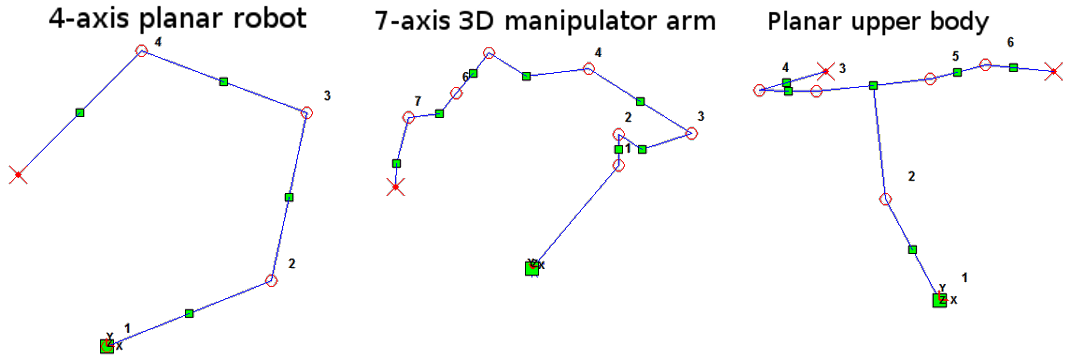
\includegraphics[width=0.98\textwidth]{robots.png}
  \caption{Examples of robots used}
\label{fig:robots}
\end{figure}

We propose to use the following test to compare the performances of different lifting methods for all our experiments:
\begin{enumerate}
  \item Choose a robot and a resolution method
  \item Generate 1000 pairs of initial configuration and end effector goal
  \item Solve the problem of finding a configuration in which the end effector reaches the goal for all the available formulations:
  \begin{itemize}
    \item Direct: Direct formulation
    \item Direct Trigo: Direct with trigonometric elimination
    \item Lifted: Lifted with maximum degree 2
    \item Lifted Trigo: Lifted with maximum degree 2 and trigonometric elimination
    \item Lifted Joint: Lifted based on joints
    \item Lifted Joint Trigo: Lifted based on joints and trigonometric elimination
  \end{itemize}
\end{enumerate}

This approach allows to fairly compare the performances of all lifting approaches on a given problem.
And to observe the influence of the number of degrees of freedom of the robot on those performances, we use the n-axis planar robot model.
We plot the average number of iterations needed to reach convergence against the number of degrees of freedom of the planar robot.
In figure~\ref{fig:lift_results} we present the results obtained for the resolution with our custom SQP, using BFGS updates and a filter line-search, without cost function, initializing all the variables randomly.
In figure~\ref{fig:lift_results2} we present the best case in favor of the lifted approach that we encountered, those results are obtained for the resolution with our custom SQP, using SR1 updates and a filter line-search, without cost function, initializing all the variables such that the lifted equations are satisfied.

\begin{figure}
\centering
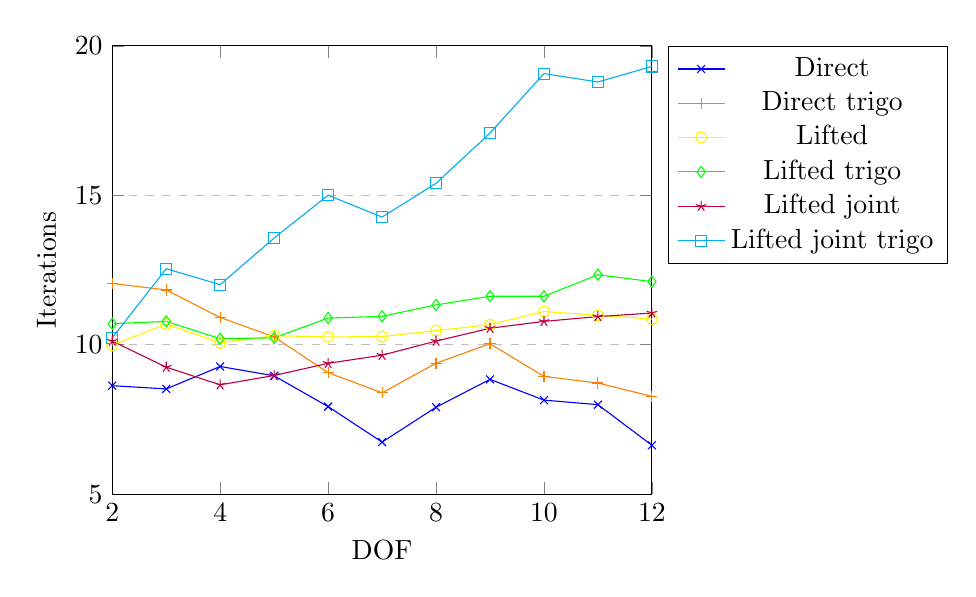
\begin{tikzpicture}
\begin{axis}[
    %title={Custom SQP, BFGS updates, filter line-search, no cost function, random initialization},
    xlabel={DOF},
    ylabel={Iterations},
    xmin=2, xmax=12,
    ymin=5, ymax=20,
    xtick={0,2,4,6,8,10,12},
    ytick={0,5,10,15,20},
    legend pos=outer north east,
    ymajorgrids=true,
    grid style=dashed,
]
\addplot[color=blue,mark=x]
    coordinates {(2,8.628)(3,8.52)(4,9.271)(5,8.958)(6,7.928)(7,6.741)(8,7.908)(9,8.84)(10,8.145)(11,7.994)(12,6.634)};
\addplot[color=orange,mark=+]
    coordinates {(2,12.05)(3,11.83)(4,10.91)(5,10.26)(6,9.063)(7,8.39)(8,9.381)(9,10.03)(10,8.94)(11,8.717)(12,8.271)};
\addplot[color=yellow,mark=o]
    coordinates {(2,9.981)(3,10.69)(4,10.06)(5,10.3)(6,10.26)(7,10.27)(8,10.47)(9,10.67)(10,11.11)(11,10.98)(12,10.86)};
\addplot[color=green,mark=diamond]
    coordinates {(2,10.7)(3,10.78)(4,10.2)(5,10.23)(6,10.89)(7,10.95)(8,11.33)(9,11.62)(10,11.62)(11,12.34)(12,12.11)};
\addplot[color=purple,mark=star]
    coordinates {(2,10.12)(3,9.248)(4,8.657)(5,8.97)(6,9.376)(7,9.649)(8,10.12)(9,10.55)(10,10.78)(11,10.94)(12,11.06)};
\addplot[color=cyan,mark=square]
    coordinates {(2,10.23)(3,12.54)(4,12.01)(5,13.57)(6,15)(7,14.27)(8,15.4)(9,17.08)(10,19.07)(11,18.79)(12,19.31)};
\legend{Direct, Direct trigo , Lifted, Lifted trigo, Lifted joint, Lifted joint trigo }
\end{axis}
\end{tikzpicture}
\caption{Number of iterations to reach convergence against number of DOF of the n-axis planar robot for the different lifting methods solved with our Custom SQP, BFGS, filter line-search, random initialization}%, no cost function
\label{fig:lift_results}
\end{figure}


\begin{figure}
\centering
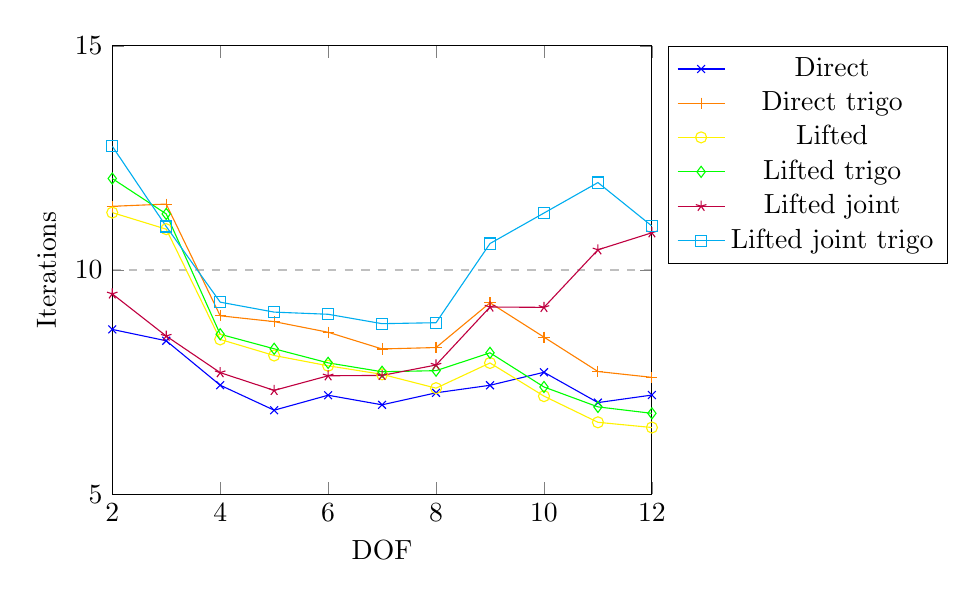
\begin{tikzpicture}
\begin{axis}[
    %title={Custom SQP, SR1 updates, filter Line-Search, no Cost, initialization satisfying lifted equations},
    xlabel={DOF},
    ylabel={Iterations},
    xmin=2, xmax=12,
    ymin=5, ymax=15,
    xtick={0,2,4,6,8,10,12},
    ytick={0,5,10,15,20},
    legend pos=outer north east,
    ymajorgrids=true,
    grid style=dashed,
]
\addplot[color=blue,mark=x]
  coordinates {(2,8.674)(3,8.421)(4,7.43)(5,6.872)(6,7.206)(7,6.992)(8,7.26)(9,7.428)(10,7.718)(11,7.042)(12,7.21)};
\addplot[color=orange,mark=+]
  coordinates {(2,11.42)(3,11.47)(4,8.978)(5,8.848)(6,8.611)(7,8.238)(8,8.27)(9,9.268)(10,8.502)(11,7.735)(12,7.605)};
\addplot[color=yellow,mark=o]
  coordinates {(2,11.28)(3,10.91)(4,8.451)(5,8.092)(6,7.863)(7,7.672)(8,7.364)(9,7.926)(10,7.186)(11,6.602)(12,6.486)};
\addplot[color=green,mark=diamond]
  coordinates {(2,12.04)(3,11.25)(4,8.566)(5,8.242)(6,7.928)(7,7.73)(8,7.754)(9,8.152)(10,7.39)(11,6.946)(12,6.802)};
\addplot[color=purple,mark=star]
  coordinates {(2,9.467)(3,8.526)(4,7.71)(5,7.314)(6,7.64)(7,7.648)(8,7.88)(9,9.174)(10,9.166)(11,10.45)(12,10.83)};
\addplot[color=cyan,mark=square]
  coordinates {(2,12.76)(3,10.97)(4,9.282)(5,9.06)(6,9.012)(7,8.802)(8,8.824)(9,10.59)(10,11.27)(11,11.95)(12,10.98)};
\legend{Direct, Direct trigo , Lifted, Lifted trigo, Lifted joint, Lifted joint trigo }
\end{axis}
\end{tikzpicture}
\caption{Number of iterations to reach convergence against number of DOF of the n-axis planar robot for the different lifting methods solved with our Custom SQP, SR1, filter Line-Search, initialization satisfying lifted equations}%, no Cost
\label{fig:lift_results2}
\end{figure}

The results presented in figure~\ref{fig:lift_results} show that the direct formulation outperforms every form of lifting for almost all the robots tested.
This is the typical result that we observed in most cases.

In figure~\ref{fig:lift_results2}, we show one specific case where, with long kinematic chains ($\geq10$ DOF), the lifted methods are slightly faster to solve.

We studied many of the possible configurations of resolution methods (22 in total), but not all of them.
Still, it seems possible to draw some conclusions out of it, because in most cases, the direct approach outperforms the lifted one.
%The only case where we observe a neat advantage in favor of the lifted methods compared to the direct one is when using the interior point method that is built-in in fmincon in Matlab with a randomized initialization and the norm 2 of the articular parameters vector as a cost function.

The overall results we extracted from those experiments is that the best performing method is: solving the direct formulation with our custom solver, using BFGS regularization and either Armijo or filter line search and no cost function.

We observed that when the lifted variables are initialized randomly the direct problem is usually solved faster than the lifted one.
Whereas when the lifted variables are initialized so that the lifted equations are initially satisfied, the results are sensibly the same for lifted and direct approaches.

After comparison of all the results that we obtained, for all the planar robots with 2 to 12 degrees of freedom and across all the resolution methods that we tried, the best performing formulation is the direct one, except for the 7 DOF robot, where the resolution of the lifted problem with maximum degree 2 outperforms slightly all the other methods.

Overall, it seems that the idea of lifting does not provide better performances than the direct formulation for solving inverse kinematics problem.
In the view of that observation, we decided to not go further in this research direction.
Even though intuitively, the idea of lifting seems to apply naturally to robotics equations, the results obtained were not satisfying enough to justify investing more efforts in this approach so we decided to move on.

\section{Conclusion}
\label{sec:chap3_conclusion}

In this chapter, we presented three different and unrelated contributions to the field.
First, we proposed a convenient formulation of contact constraints that allows generating non-inclusive contacts between two surfaces while ensuring that the size of the intersection is satisfactory.
Second, we presented a generic differentiation of the torque computation algorithm, allowing to compute the joint torque jacobian of a robotic system.
And finally, we described our endeavor to use the idea of variable lifting in optimization to solve posture generation problems, which unfortunately proved inefficient to accelerate the convergence of our solvers on those problems.

In the next chapter, we will dive deeper in the field of nonlinear optimization on manifolds, study how an SQP algorithm can be modified to be able to deal with manifolds and finally present our own implementation of such an algorithm.
